% Se compila con XeLaTeX; hacen falta varias pasadas para que se resuelvan las referencias.
\documentclass[11pt,a4paper]{article}
\usepackage{fontspec}
\IfFontExistsTF{texgyrepagella-regular.otf}
 {\setmainfont{texgyrepagella}[Extension=.otf,UprightFont=*-regular,BoldFont=*-bold,
   ItalicFont=*-italic,BoldItalicFont=*-bolditalic]}
 {\IfFontExistsTF{Palatino Linotype}{\setmainfont{Palatino Linotype}}{\setmainfont{Latin Modern Roman}}}
\linespread{1.05}
% Con babel-spanish instalado (MiKTeX, TeX Live completo) se usa la opción clásica; si falta,
% se carga el locale español de babel sin patrones de guionado.
\IfFileExists{spanish.ldf}
 {\usepackage[spanish,es-noshorthands,es-nodecimaldot,es-tabla]{babel}}
 {\usepackage{babel}\babelprovide[import,main,hyphenrules=nohyphenation]{spanish}}
\usepackage{amsmath,amssymb,amsthm,mathtools}
\usepackage{unicode-math}
\IfFontExistsTF{texgyrepagella-math.otf}{\setmathfont{texgyrepagella-math.otf}}{\setmathfont{Latin Modern Math}}
\usepackage[margin=26mm]{geometry}
\IfFileExists{microtype.sty}{\usepackage{microtype}}{}
\IfFileExists{titlesec.sty}{\usepackage[nobottomtitles*]{titlesec}
  \renewcommand{\bottomtitlespace}{.12\textheight}}{}
\usepackage{booktabs,array}
\usepackage[shortlabels]{enumitem}
\usepackage{tikz}
\usetikzlibrary{arrows.meta,positioning}
\usepackage{xcolor}
\usepackage[colorlinks=true,linkcolor={blue!45!black},citecolor={green!35!black},urlcolor={blue!55!black}]{hyperref}

\AtBeginDocument{\renewcommand{\tablename}{Tabla}}
\setlength{\parskip}{3pt}
\setlength{\emergencystretch}{2em}
\allowdisplaybreaks[2]
\numberwithin{equation}{section}

\theoremstyle{plain}
\newtheorem{teorema}{Teorema}[section]
\newtheorem{proposicion}[teorema]{Proposición}
\newtheorem{lema}[teorema]{Lema}
\newtheorem{corolario}[teorema]{Corolario}
\theoremstyle{definition}
\newtheorem{definicion}[teorema]{Definición}
\theoremstyle{remark}
\newtheorem{observacion}[teorema]{Observación}

% Notación
\newcommand{\ind}{\mathbf{1}}
\DeclareMathOperator{\Lip}{Lip}
\newcommand{\cA}{{\mathcal{A}}}
\newcommand{\cH}{{\mathcal{H}}}
\newcommand{\cE}{{\mathcal{E}}}
\newcommand{\cG}{{\mathcal{G}}}
\newcommand{\sopt}{s^{*}}

\title{El perfil variacional de las colocaciones parciales de reinas:\\[3pt]
\large Existencia, ecuaciones de Euler y regularidad hasta el tablero lleno}
\author{Dilan Steven Mejia\thanks{\href{mailto:mejiadilan@hotmail.com}{\nolinkurl{mejiadilan@hotmail.com}}}}
\date{}
\hypersetup{pdftitle={El perfil variacional de las colocaciones parciales de reinas: existencia, ecuaciones de Euler y regularidad hasta el tablero lleno},pdfauthor={Dilan Steven Mejia},
 pdfsubject={Problema variacional de las n reinas. MSC 2020: 49K27, 05A16, 46N10, 94A17},
 pdfkeywords={problema de las n reinas, entropía variacional, ecuaciones de Euler,
  regularidad espacial},
 pdflang={es}}
% DOI de Zenodo del repositorio de verificación numérica, sin «https://doi.org/»
% (por ejemplo 10.5281/zenodo.1234567). Mientras esté vacío, el artículo no cita el repositorio.
\newcommand*{\DOIcodigo}{}
\ifx\DOIcodigo\empty\typeout{AVISO: falta el DOI del repositorio numerico (DOIcodigo).}\fi
\begin{document}
\maketitle
\begin{abstract}
\noindent Una colocación de reinas tiene a lo sumo una reina en cada fila, columna y diagonal de ambas direcciones.
Estudiamos el problema continuo de maximizar la entropía de una densidad de masa
$\rho$ en el cuadrado unidad bajo estas cuatro restricciones. Para $\rho=1$ el funcional es el del problema variacional
de Simkin para las $n$ reinas. Para $0<\rho<1$, el maximizador es único
y su densidad en cada punto, salvo en un conjunto de medida cero, es proporcional al producto de
las capacidades restantes de las cuatro líneas que pasan por él; la constante de proporcionalidad
$\lambda(\rho)$ es la actividad.
Al acercarse la masa a uno, la capacidad restante de filas y columnas tiende a cero.
Al dividirla por $x=1-\rho$ obtenemos perfiles positivos que convergen uniformemente
y, junto con las capacidades restantes de las diagonales y el límite de la actividad reescalada $\lambda x^2$, determinan el maximizador de masa uno. Estos perfiles dependen analíticamente de $x$ cerca de cero
y satisfacen una cota Lipschitz espacial uniforme hasta el tablero lleno.
La actividad $\lambda(\rho)$ del maximizador determina la función
$F(x)=(1-x)/(\lambda(1-x)x^2)$, que se extiende analíticamente a ambos extremos y cumple
$\int_0^1\log F(x)\,dx=1+s^*(1)$, donde $s^*(1)$ es la entropía óptima en masa uno; además,
$s^*(1-x)-s^*(1)=2x\log(1/x)+O(x)$. Una extrapolación numérica, sin certificación de error,
da $F(0)\approx0{,}0809$ y $s^*(1)\approx-1{,}9440$, compatible con los valores conocidos de la
constante de Simkin. Todos los resultados se refieren al problema continuo.
\end{abstract}
\noindent\small\textbf{Palabras clave.} Problema de las $n$ reinas, entropía variacional,
ecuaciones de Euler, regularidad espacial. \quad\textbf{MSC 2020.} 49K27, 05A16, 46N10, 94A17.\par\normalsize
\section{Introducción}\label{sec:intro}

El problema de las $n$ reinas consiste en colocar $n$ reinas en un tablero de $n\times n$
sin que dos compartan fila, columna ni diagonal de ninguna de las dos direcciones.
Cuando sólo hemos colocado $q$ reinas, quedan exactamente $n-q$ filas y $n-q$ columnas vacías.
En un tablero de $5\times5$ con cuatro reinas, por ejemplo, la fila y la columna que faltan
determinan una única casilla candidata. En la Figura~\ref{fig:tablero-fibras}(a)
también están libres sus dos diagonales, por lo que allí cabe la quinta reina.
Numeramos filas y columnas desde cero y escribimos primero la fila.

\begin{figure}[htbp]
\centering
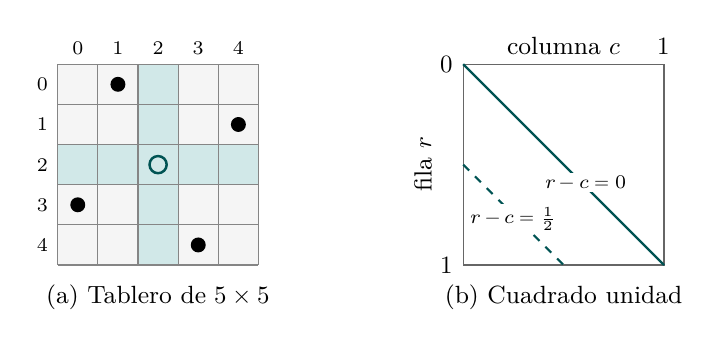
\begin{tikzpicture}[font=\small]
\begin{scope}[x=.51cm,y=-.51cm]
  \fill[black!4] (0,0) rectangle (5,5);
  \fill[teal!18] (0,2) rectangle (5,3);
  \fill[teal!18] (2,0) rectangle (3,5);
  \foreach \i in {0,...,5}{
    \draw[black!48,thin] (0,\i) -- (5,\i);
    \draw[black!48,thin] (\i,0) -- (\i,5);
  }
  \foreach \i in {0,...,4}{
    \node[left] at (0,\i+.5) {\scriptsize\i};
    \node[above] at (\i+.5,0) {\scriptsize\i};
  }
  \foreach \r/\c in {0/1,1/4,3/0,4/3}{
    \fill (\c+.5,\r+.5) circle[radius=2.7pt];
  }
  \draw[teal!65!black,line width=.9pt] (2.5,2.5) circle[radius=3.1pt];
  \node[anchor=north] at (2.5,5.25) {(a) Tablero de $5\times5$};
\end{scope}
\begin{scope}[shift={(5.15,0)},x=2.55cm,y=-2.55cm]
  \draw[black!60] (0,0) rectangle (1,1);
  \draw[teal!65!black,thick] (0,0) -- (1,1);
  \draw[teal!65!black,thick,dashed] (0,.5) -- (.5,1);
  \node[fill=white,inner sep=1pt,font=\scriptsize] at (.61,.59) {$r-c=0$};
  \node[fill=white,inner sep=1pt,font=\scriptsize] at (.25,.77) {$r-c=\tfrac12$};
  \node[left] at (0,0) {$0$}; \node[left] at (0,1) {$1$};
  \node[above] at (1,0) {$1$};
  \node[above] at (.50,0) {columna $c$};
  \node[rotate=90] at (-.20,.50) {fila $r$};
  \node[anchor=north] at (.5,1.05) {(b) Cuadrado unidad};
\end{scope}
\end{tikzpicture}
\caption{Del tablero a las líneas del cuadrado. En (a), cada punto negro es una reina.
La fila~2 y la columna~2 están libres. El círculo señala su intersección.
En (b), cada valor de $r-c$ identifica una diagonal. La longitud de su proyección
sobre el eje de filas vale uno para la línea continua y un medio para la discontinua.}
\label{fig:tablero-fibras}
\end{figure}

Asignemos a cada reina una masa $1/n$. La colocación tiene masa total $\rho=q/n$,
y $x=1-\rho$ es la fracción de filas vacías, que coincide con la de columnas vacías.
En el ejemplo, $x=1/5$. Al pasar al cuadrado unidad, podemos preguntar cómo se distribuye
la masa si conservamos la restricción de capacidad de cada familia de líneas.
En un tablero lleno ($\rho=1$, $x=0$) las filas y las columnas agotan su capacidad. ¿Qué información sobre
su distribución se conserva cuando nos acercamos a ese extremo desde las masas parciales?

En masa uno, Simkin~\cite{Simkin} relacionó la entropía de un perfil del cuadrado con
el número $Q(n)$ de soluciones y obtuvo $Q(n)=((1+o(1))\,n\,e^{-\alpha})^n$.
Nobel, Agrawal y Boyd~\cite{NAB} situaron $\alpha$ entre $1{,}944000752$ y $1{,}944001082$.
Aquí estudiamos cómo varía el perfil que maximiza la entropía a medida que $\rho$ crece hacia uno.
Para distinguir dos filas cuya capacidad restante tiende a cero, mediremos qué parte
de la vacancia total corresponde a cada una.

\subsection{El problema continuo}


Sea $[0,1]^2$ el cuadrado, con coordenadas $(r,c)$ de fila y columna. Las cuatro familias de líneas
son las filas, columnas, diagonales y antidiagonales, con proyecciones
\[
 \ell_R(r,c)=r,\qquad \ell_C(r,c)=c,\qquad \ell_D(r,c)=r-c,\qquad \ell_A(r,c)=r+c,
\]
que toman valores en $I_R=I_C=[0,1]$, $I_D=[-1,1]$ e $I_A=[0,2]$. Para una densidad $\nu\ge0$ en
el cuadrado, $m_f$ denota su proyección sobre la familia $f$ y $u_f=1-m_f$ su \emph{vacancia}
o capacidad restante. Por ejemplo, $m_R(r)$ se obtiene integrando $\nu(r,c)$ respecto de $c$ a lo largo de la fila $r$.
En una diagonal la integral sólo recorre el segmento que cae dentro del cuadrado
(Figura~\ref{fig:tablero-fibras}(b) y Sección~\ref{sec:preliminares}). Para $\rho\in(0,1]$, la clase admisible $\cA_\rho$ está formada por
las densidades de masa $\rho$ con $m_f\le1$ en casi todo punto para las cuatro familias, y
\begin{equation}\label{eq:funcional}
 s[\nu]=-3\rho-\int_{[0,1]^2}\nu\log\nu-\sum_{f\in\{R,C,D,A\}}\int_{I_f}u_f\log u_f,\qquad
 \sopt(\rho)=\sup_{\nu\in\cA_\rho}s[\nu].
\end{equation}

El primer término integral mide cómo se reparte la masa en el cuadrado. Los otros cuatro
términos registran cómo se distribuye la capacidad restante dentro de cada
familia. En masa uno, las vacancias de filas y columnas son nulas y $s$ coincide con la
entropía del problema de Simkin (Observación~\ref{obs:simkin}). Llamaremos \emph{perfil óptimo} a la densidad que maximiza $s$
para una masa dada, junto con sus cuatro proyecciones.

\subsection{Resultados principales}

\begin{teorema}[Maximizador y ecuación de Euler]\label{thm:euler}
Para cada $\rho\in(0,1)$, $s$ alcanza su supremo en $\cA_\rho$ en una única densidad $\nu_\rho$, y
existe $\lambda=\lambda(\rho)>0$ tal que
\[
 \nu_\rho=\lambda\prod_f u_f\circ\ell_f\quad\text{en casi todo punto},\qquad
 \frac{\lambda}{(1+\lambda)^4}\le\nu_\rho\le\lambda,\qquad m_f\le\frac{\lambda}{1+\lambda}.
\]
La función $\sopt$ es estrictamente cóncava y derivable en $(0,1)$, con $\sopt{}'(\rho)=-\log\lambda(\rho)$;
$\lambda$ es continua y estrictamente creciente, $\lambda\to0$ cuando $\rho\to0$ y $\lambda\to\infty$
cuando $\rho\to1$. Para $\rho=1$ el supremo también se alcanza en una única densidad $\nu_1$.
\end{teorema}

La ecuación de Euler liga la densidad en una casilla a la capacidad restante de
las cuatro líneas que la atraviesan. La constante $\lambda$, que llamaremos \emph{actividad}, ajusta la masa total.
Cuando $\rho$ tiende a uno, $\lambda$ crece sin cota y las dos vacancias de filas y
columnas tienen integral $x$. Para conservar su distribución espacial escribimos,
con $\rho=1-x\in(0,1)$,
\begin{equation}\label{eq:reescala}
 r_R=\frac{u_R}x,\qquad r_C=\frac{u_C}x,\qquad b=\lambda x^2,
\end{equation}
de modo que $\nu=b\,r_R\,r_C\,u_D\,u_A$ e $\int_0^1r_R=\int_0^1r_C=1$.

\begin{teorema}[El perfil cerca del tablero lleno]\label{thm:lleno}
Existen constantes explícitas $0<\kappa\le1$, $1\le M<\infty$ y $0<b_+<\infty$ tales que, para
todo $x\in(0,1/2]$,
\[
 \tfrac12\le b\le b_+,\qquad \frac1{1+b_+}\le r_R,r_C\le M,\qquad \kappa\le u_D,u_A\le1 .
\]
Cuando $x\downarrow0$, $(b,r_R,r_C,u_D,u_A)$ converge uniformemente a un límite
$(b_0,r_{R,0},r_{C,0},u_{D,0},u_{A,0})$ formado por funciones continuas y positivas, con
$\nu_1=b_0\,r_{R,0}\,r_{C,0}\,u_{D,0}\,u_{A,0}$, y la aplicación
$x\mapsto(\log r_R,\log r_C,\log u_D,\log u_A,\log b)$, con valores en
$\bigoplus_fC(I_f)\times\mathbb R$, se extiende analíticamente a un entorno de $x=0$.
\end{teorema}

El teorema anterior describe qué ocurre al cambiar la masa. También necesitamos
comparar dos posiciones de un mismo tablero. Una cota Lipschitz controla el cambio
del perfil por la distancia entre esas posiciones. La cuestión es si la misma
constante sigue sirviendo cuando quedan cada vez menos filas vacías.

\begin{teorema}[Regularidad espacial]\label{thm:lipschitz_intro}
\begin{enumerate}[(a)]
\item Para $\rho\in(0,1)$ y $\lambda=\lambda(\rho)$, las vacancias y las proyecciones son Lipschitz en
sus intervalos cerrados con constante $L(\lambda)=2\lambda+8\lambda^2(1+\lambda)$, y $\nu_\rho$ es
Lipschitz en el cuadrado con constante $6\lambda L(\lambda)$ para la norma del máximo. Las cotas son
uniformes en cada compacto de $(0,1)$.
\item Existe $L_*<\infty$ tal que, para todo $x\in[0,1/2]$, los factores reescalados
$r_R,r_C,u_D,u_A$ son Lipschitz con constante $L_*$, y $\nu$ es acotada y Lipschitz con constantes
independientes de $x$.
\end{enumerate}
\end{teorema}

La parte (a) degenera cuando $\rho\to1$, porque $\lambda(\rho)\to\infty$; la parte (b) es la que
permite trabajar hasta el tablero lleno.

Definimos, para $x\in(0,1)$ y $\rho=1-x$,
\begin{equation}\label{eq:F}
 F(x)=\frac{1-x}{\lambda(1-x)\,x^2}=\frac{1-x}{b}=\int_{[0,1]^2}r_R(r)\,r_C(c)\,u_D(r-c)\,u_A(r+c)\,dr\,dc .
\end{equation}
La última expresión es la integral de $u_D(r-c)\,u_A(r+c)$ respecto del peso $r_R(r)\,r_C(c)$,
que es una densidad de probabilidad en el cuadrado. El interés de $F$ está en la identidad
integral del teorema siguiente, que recupera $\sopt(1)$ a partir de ella.

\begin{teorema}[La función $F$ y el valor óptimo]\label{thm:F_intro}
La función $F$ se extiende a una función real analítica y positiva en un entorno de $[0,1]$, con
\[
 F(0)=\frac1{b_0},\qquad F(1)=1,\qquad \int_0^1\log F(x)\,dx=1+\sopt(1).
\]
Además, cuando $x\downarrow0$,
\[
 \sopt(1-x)-\sopt(1)=2x\log\frac1x+O(x).
\]
\end{teorema}

\begin{observacion}[Valores numéricos]
Una resolución numérica determinista del sistema de Euler (Sección~\ref{sec:discusion}) da
$F(0)\approx0{,}0809$, $F'(0)\approx0{,}516$ e $\int_0^1\log F\approx-0{,}9440$, de modo que
$\sopt(1)\approx-1{,}9440$. Este valor es compatible con los valores conocidos de la constante
$\alpha$~\cite{Simkin,NAB}, como cabe esperar si $\alpha=-\sopt(1)$
(véase la Observación~\ref{obs:simkin}). Son valores numéricos, sin
certificación de error.
\end{observacion}

\subsection{Del maximizador al perfil límite}

Para la masa uno, la existencia y la unicidad del óptimo de la entropía
figuran en el Lema~2.22 de Simkin~\cite{Simkin}. La
Observación~\ref{obs:simkin} precisa la correspondencia de los funcionales.
La familia de masas parciales permite estudiar cómo se llega a ese óptimo.
Primero deducimos la ecuación de Euler en el interior (Sección~\ref{sec:euler}).
Sus cotas reescaladas permiten identificar los factores que subsisten en masa uno
(Secciones~\ref{sec:cotas} y~\ref{sec:limite}). El análisis de la dependencia
respecto de la masa se completa en la Sección~\ref{sec:analiticidad}.
Para controlar los cambios de posición comparamos el perfil con sus traslaciones
(Sección~\ref{sec:regularidad}). Finalmente, al integrar la ecuación de Euler
se obtiene la relación entre $F$ y la entropía óptima (Sección~\ref{sec:F}),
que evaluamos numéricamente en la Sección~\ref{sec:discusion}.

\subsection{Relación con trabajos previos}

Simkin~\cite{Simkin} acota el valor óptimo en masa uno discretizando el problema; su cota
superior usa la dualidad de Lagrange, que da al maximizador discreto una forma exponencial en los
multiplicadores~\cite[Sección~6]{Simkin}. Nobel, Agrawal y Boyd~\cite{NAB} resuelven una
discretización del mismo problema con un método de Newton y obtienen el intervalo citado. Que el
maximizador de una entropía bajo restricciones lineales tenga forma exponencial es un principio
clásico~\cite{Csiszar}. Lo que añade este trabajo es el estudio de la familia de masas parciales,
con su ecuación de Euler, y sobre todo el control uniforme hasta el tablero lleno: cotas
explícitas, convergencia y analiticidad del perfil reescalado, regularidad Lipschitz uniforme y
la identidad integral para $F$. Hasta donde sabemos, estos resultados son nuevos; no se reclama novedad para las técnicas generales de
análisis convexo, de dualidad y de la función implícita~\cite{Brezis,Zeidler}.

\section{Preliminares}\label{sec:preliminares}

\subsection{Proyecciones y fibras}

Extendemos cada densidad $\nu\ge0$ integrable en $[0,1]^2$ por cero fuera del cuadrado. Sus
proyecciones (o densidades de línea) son
\begin{gather*}
 m_R(r)=\int_0^1\nu(r,c)\,dc,\qquad m_C(c)=\int_0^1\nu(r,c)\,dr,\\
 m_D(d)=\int\nu(r,r-d)\,dr,\qquad m_A(s)=\int\nu(r,s-r)\,dr,
\end{gather*}
definidas en casi todo punto de $I_R,I_C,I_D,I_A$. Escribimos también $T_f\nu=m_f$. La \emph{fibra}
de $f$ en $t\in I_f$ es $\{\ell_f=t\}\cap[0,1]^2$, con la medida paramétrica $dc$ para las filas y
$dr$ para las demás familias, sin el factor $\sqrt2$ de la longitud euclídea. Toda fibra tiene
longitud paramétrica a lo sumo uno: la diagonal $d$ mide $1-|d|$ y la antidiagonal $s$, $1-|s-1|$.

\begin{lema}\label{lem:fubini}
Para toda $g\ge0$ medible en $I_f$, $\int_{[0,1]^2}\nu\,(g\circ\ell_f)=\int_{I_f}m_f\,g$. En
particular $\int_{I_f}m_f=\int\nu$ para las cuatro familias, y
$\|T_f\nu-T_f\nu'\|_{L^1(I_f)}\le\|\nu-\nu'\|_{L^1}$.
\end{lema}

\begin{proof}
Es el teorema de Fubini con los cambios de variable $(r,c)\mapsto(r,\ell_f(r,c))$ o
$(r,c)\mapsto(c,\ell_f(r,c))$, de jacobiano uno.
\end{proof}

La densidad constante $\nu=\rho$ permite leer estas integrales en la Figura~\ref{fig:tablero-fibras}(b).
La diagonal central recoge masa $\rho$ por unidad de coordenada diagonal y la de
$r-c=1/2$ recoge $\rho/2$, pues su intervalo de filas tiene la mitad de longitud.
Así, aun con densidad constante en el cuadrado, la proyección diagonal varía con la posición.

\subsection{La clase admisible y el funcional}

Las vacancias son $u_f=1-m_f$. Para $\rho\in(0,1]$, $\cA_\rho$ es el conjunto de las densidades
$\nu\ge0$ con $\int\nu=\rho$ y $m_f\le1$ en casi todo punto para las cuatro familias. Por el
Lema~\ref{lem:fubini}, $\int u_R=\int u_C=1-\rho$ e $\int u_D=\int u_A=2-\rho$. Con
$G(z)=-(1-z)\log(1-z)$ en $[0,1]$ y $0\log0=0$, el funcional~\eqref{eq:funcional} se escribe
\[
 s[\nu]=-3\rho-\int\nu\log\nu+\sum_f\int_{I_f}G(m_f),
\]
con $s[\nu]=-\infty$ si $\int\nu\log\nu=+\infty$. La función $G$ es cóncava, continua y
$0\le G\le1/e$. Escribimos
\[
 \Pi[\nu](r,c)=\prod_f\bigl(1-m_f(\ell_f(r,c))\bigr)=\prod_fu_f(\ell_f(r,c)).
\]

\begin{lema}[Propiedades elementales]\label{lem:elementales}
\begin{enumerate}[(a)]
\item $\cA_\rho$ es convexo y cerrado en $L^1$, y $s$ es cóncavo en $\cA_\rho$; el término
$-\int\nu\log\nu$ es estrictamente cóncavo.
\item Para $\rho<1$, la densidad constante $\rho$ pertenece a $\cA_\rho$, con proyecciones $\rho$,
$\rho$, $\rho(1-|d|)$ y $\rho(1-|s-1|)$.
\item $s\le-\rho\log\rho+6/e$ en $\cA_\rho$; en particular $\sopt(\rho)<\infty$.
\end{enumerate}
\end{lema}

\begin{proof}
(a) La masa y las proyecciones son lineales; la cerradura sigue del Lema~\ref{lem:fubini}. La
concavidad de $G$ y de $-z\log z$ da la de $s$. (b) Es un cálculo directo. (c) Por Jensen,
$-\int\nu\log\nu\le-\rho\log\rho$, y los dominios de las cuatro familias miden en total seis, con
$G\le1/e$.
\end{proof}

\begin{observacion}[Relación con el problema de Simkin]\label{obs:simkin}
Para $\rho=1$, las proyecciones de filas y columnas valen uno y $u_R=u_C=0$, de modo que
$s[\nu]=-3-\int\nu\log\nu-\int u_D\log u_D-\int u_A\log u_A$. Tras trasladar el cuadrado a
$[-\frac12,\frac12]^2$, las vacancias diagonales son densidades de integral uno en intervalos de
longitud dos, y cada divergencia respecto de la uniforme en $[-1,1]$ vale $\int u\log u+\log2$. En la Definición~2.9 de~\cite{Simkin}, las dos constantes $\log2$ se cancelan con el
término $2\log2$. Se obtiene así la misma expresión para la entropía sobre las densidades
admisibles de masa uno. La Observación~2.7 de esa referencia distingue la clase de medidas
definida por las restricciones de proyección y la definida por clausura, y precisa su relación
para las medidas absolutamente continuas. Según la Sección~2.2 de~\cite{Simkin} (Teorema~2.24,
aplicado a toda la clase definida por clausura, y Lema~2.22), $-\alpha$ es el máximo de esa entropía
en dicha clase. Con la correspondencia anterior y la Observación~2.7 citada se seguiría
$\alpha=-\sopt(1)$. Esa identidad no se usa en este trabajo, y la comparación de constantes de la
Sección~\ref{sec:discusion} es numérica.
\end{observacion}

\begin{observacion}[Una densidad estrictamente admisible de masa uno]\label{obs:slater}
La densidad $\nu^\sharp(r,c)=1-\frac15\cos(2\pi r)\cos(2\pi c)$ cumple $\frac45\le\nu^\sharp\le\frac65$ y
tiene proyecciones de filas y columnas idénticamente iguales a uno. Para $0\le d\le1$,
\[
 m_D[\nu^\sharp](d)=1-d-\frac15\Bigl[\frac{1-d}2\cos(2\pi d)-\frac{\sin(2\pi d)}{4\pi}\Bigr],
\]
cuya derivada es $-1+\frac15[\cos(2\pi d)+\pi(1-d)\sin(2\pi d)]\le-1+\frac{1+\pi}5<0$; como
$m_D[\nu^\sharp](0)=\frac9{10}$, se obtiene $m_D[\nu^\sharp]\le\frac9{10}$. Por simetría, lo mismo vale para
$d<0$ y para la familia antidiagonal. En particular $\nu^\sharp\in\cA_1$ y $s[\nu^\sharp]>-\infty$.
\end{observacion}

\section{Existencia, unicidad y ecuación de Euler}\label{sec:euler}

A masa fija, tanto la densidad como sus cuatro proyecciones intervienen en la entropía.
La concavidad estricta del término $-\int\nu\log\nu$ asegura que hay a lo sumo un óptimo. Para averiguar su forma,
primero justificamos que existe y que ninguna capacidad se satura en un conjunto
de medida positiva. Entonces podemos variar la densidad y deducir la ecuación de Euler.

\begin{teorema}\label{thm:max}
Sea $0<\rho<1$.
\begin{enumerate}[(a)]
\item $s$ alcanza su supremo en $\cA_\rho$ en una única densidad $\nu_\rho$.
\item Existe $\theta=\theta(\rho)\in\mathbb R$ tal que $\nu_\rho=e^{-\theta}\,\Pi[\nu_\rho]$ en casi todo
punto.
\item Sea $\lambda=e^{-\theta}$ (la \emph{actividad}). Las cuatro proyecciones de $\nu_\rho$ son $\le\lambda/(1+\lambda)$, se
tiene $\lambda(1+\lambda)^{-4}\le\nu_\rho\le\lambda$, y $\rho=\lambda\int\Pi[\nu_\rho]$.
\item Para todo $\rho'\in(0,1)$, $\sopt(\rho')\le\sopt(\rho)+\theta(\rho)(\rho'-\rho)$. En
particular $\sopt$ es cóncava, $\theta$ es no creciente y $\lambda$ no decreciente. Además $\sopt$ es
derivable, con $\sopt{}'=\theta$, y $\theta$ es continua.
\end{enumerate}
\end{teorema}

\begin{proof}
Escribimos $\nu^*=\nu_\rho$ y $m^*_f$, $u^*_f$ para sus proyecciones y vacancias.

\emph{Paso 1: existencia y unicidad.} Sea $(\nu_k)\subset\cA_\rho$ con $s[\nu_k]\to\sopt(\rho)$.
Como los términos de línea están acotados por $6/e$, $\int\nu_k\log\nu_k$ está acotada; por los
criterios de de la Vallée-Poussin y Dunford--Pettis~\cite{Bogachev}, una subsucesión converge
débilmente en $L^1$ a una $\nu^*$. El conjunto $\cA_\rho$ es convexo y cerrado en $L^1$, luego
débilmente cerrado, y $\nu^*\in\cA_\rho$. El funcional $s$ es cóncavo y semicontinuo superiormente en
$L^1$: la entropía por Fatou, pues $z\log z\ge-1/e$, y los términos de línea son continuos por
convergencia dominada, pues $G$ es continua y acotada. Por el lema de Mazur su hipógrafo es
débilmente cerrado~\cite{Brezis}, así que $s[\nu^*]\ge\limsup s[\nu_k]=\sopt(\rho)$. La unicidad sale
de la concavidad estricta de la entropía.

\emph{Paso 2: derivadas laterales.} Sea $\nu\in\cA_\rho$ con $s[\nu]>-\infty$ y
$\varphi(t)=s[\nu^*+t(\nu-\nu^*)]$, $t\in[0,1]$. Es cóncava y máxima en $t=0$, así que
$\varphi'(0^+)\le0$. Cada término de $s$ es cóncavo en $t$; sus cocientes incrementales en $0$ crecen
cuando $t\downarrow0$ y están acotados inferiormente por el cociente en $t=1$, que es integrable. Por
convergencia monótona, con $\log0=-\infty$,
\[
 \varphi'(0^+)=-\int(\nu-\nu^*)(\log\nu^*+1)+\sum_f\int_{I_f}(m_f-m^*_f)\bigl(\log u^*_f+1\bigr),
\]
donde cada término está en $(-\infty,+\infty]$; el término $-3\rho$ no contribuye porque las masas
son iguales.

\emph{Paso 3: $\nu^*>0$ y $m^*_f<1$ en casi todo punto.} Tomemos $\nu\equiv\rho$. Si $\{\nu^*=0\}$
tuviera medida positiva, el primer integrando valdría $+\infty$ allí y $\varphi'(0^+)=+\infty$. Si
$\{m^*_f=1\}$ tuviera medida positiva, el término de la familia $f$ valdría $+\infty$, porque las
proyecciones de $\nu\equiv\rho$ son menores que uno. Ambas cosas contradicen $\varphi'(0^+)\le0$.

\emph{Paso 4: integrabilidad.} Con $\nu\equiv\rho$, cada término de $\varphi'(0^+)$ es finito, pues
todos son $>-\infty$ y su suma es $\le0$. En el término de $f$, donde
$m^*_f>\max\{(1+\rho)/2,\,1-1/e\}$ el integrando es $\ge\frac{1-\rho}2(-\log u^*_f-1)\ge0$, y en el
resto está acotado; por eso $\int_{I_f}m^*_f|\log u^*_f|<\infty$. También
$\int\nu^*|\log\nu^*|<\infty$, porque la entropía de $\nu^*$ es finita. Sea
\[
 W=-\log\nu^*+\sum_f\log\bigl(u^*_f\circ\ell_f\bigr),
\]
finita en casi todo punto. Por lo anterior y el Lema~\ref{lem:fubini}, $\nu^*W\in L^1$; sea
$\theta=\rho^{-1}\int\nu^*W$. Si $\int\nu|\log\nu^*|$ y las
$\int\nu|\log u^*_f\circ\ell_f|$ son finitas, los términos del paso~2 se trasladan al cuadrado y,
como las masas son iguales, las constantes se cancelan: $\varphi'(0^+)=\int(\nu-\nu^*)W$.

\emph{Paso 5: $W\le\theta$ en casi todo punto.} Si no, existen $\varepsilon,\gamma>0$ y $N<\infty$
tales que el conjunto $E$ de los puntos con $\theta+\varepsilon<W\le N$ y con sus cuatro líneas de
proyección $m^*_f\le1-\gamma$ tiene medida positiva, porque $W$ es finita y $m^*_f\circ\ell_f<1$ en
casi todo punto. En $E$, $|\log\nu^*|\le|\theta|+\varepsilon+|N|+4\log\frac1\gamma$ y
$|\log u^*_f\circ\ell_f|\le\log\frac1\gamma$. Sea $g=\frac\rho{|E|}\ind_E$ y
$\nu_\tau=(1-\tau)\nu^*+\tau g$. Si una línea corta a $E$, la proyección de $\nu^*$ en ella es
$\le1-\gamma$ y la de $g$ es $\le\rho/|E|$; si no lo corta, $g$ no contribuye. Así
$\nu_\tau\in\cA_\rho$ para $\tau\le\gamma|E|/\rho$, con $s[\nu_\tau]>-\infty$, y por el paso~4
\[
 \varphi'(0^+)=\tau\Bigl(\frac\rho{|E|}\int_EW-\int\nu^*W\Bigr)\ge\tau\bigl(\rho(\theta+\varepsilon)-\rho\theta\bigr)>0,
\]
contra $\varphi'(0^+)\le0$.

\emph{Paso 6: la ecuación.} Por el paso~5, $\int\nu^*(\theta-W)=0$ con integrando $\ge0$; luego
$\nu^*(\theta-W)=0$ en casi todo punto y, como $\nu^*>0$, $W=\theta$. Es decir,
$\nu^*=e^{-\theta}\,\Pi[\nu^*]$.

\emph{Paso 7: las cotas.} Por la ecuación y el Lema~\ref{lem:fubini}, para casi todo $r\in I_R$,
\[
 m^*_R(r)=\lambda\,u^*_R(r)\int_0^1u^*_C(c)\,u^*_D(r-c)\,u^*_A(r+c)\,dc\ \le\ \lambda\bigl(1-m^*_R(r)\bigr),
\]
de donde $m^*_R\le\lambda/(1+\lambda)$. Para las otras familias es igual: la integral recorre una
fibra de longitud paramétrica $\le1$. Entonces cada factor de $\Pi[\nu^*]$ está entre
$1/(1+\lambda)$ y $1$, lo que da $\lambda(1+\lambda)^{-4}\le\nu^*\le\lambda$. Integrando la ecuación,
$\rho=\lambda\int\Pi[\nu^*]$.

\emph{Paso 8: supergradiente.} Sean $\rho'\in(0,1)$, $\nu'\in\cA_{\rho'}$ con $s[\nu']>-\infty$ y
$\varphi(t)=s[\nu^*+t(\nu'-\nu^*)]$, cóncava en $[0,1]$. Por el paso~7, $\log\nu^*$ y los
$\log u^*_f$ están acotados, así que el cálculo del paso~2 vale con todos los términos finitos.
Ahora las masas difieren, pero las constantes vuelven a cancelarse: $-(\rho'-\rho)$ de la entropía,
$+4(\rho'-\rho)$ de las cuatro familias y $-3(\rho'-\rho)$ del término $-3\rho$. Queda
$\varphi'(0^+)=\int(\nu'-\nu^*)W=\theta(\rho'-\rho)$, y $s[\nu']=\varphi(1)\le\varphi(0)+\varphi'(0^+)$.
Tomando el supremo en $\nu'$ sale la desigualdad de~(d). Una función que en cada punto queda por
debajo de una recta que la toca es cóncava. Si $\rho_1<\rho_2$, sumando las desigualdades en $\rho_1$
y en $\rho_2$ queda $(\theta(\rho_1)-\theta(\rho_2))(\rho_2-\rho_1)\ge0$.

\emph{Paso 9: la derivada.} Si $|\sigma-1|$ es pequeño, $\sigma\nu^*\in\cA_{\sigma\rho}$, porque
sus proyecciones son $\le\sigma\lambda/(1+\lambda)<1$. La función
\[
 \psi(\sigma)=s[\sigma\nu^*]=-3\sigma\rho-\sigma\int\nu^*\log\nu^*-\sigma\rho\log\sigma+\sum_f\int_{I_f}G(\sigma m^*_f)
\]
es de clase $C^2$ cerca de $\sigma=1$, con $\psi'(1)=\int\nu^*W=\rho\theta$ y
$|\psi''(\sigma)|\le\rho/\sigma+\sum_f\int(m^*_f)^2/(1-\sigma m^*_f)$, que está acotada. Entonces
$\sopt(\rho+h)\ge\psi(1+h/\rho)\ge\sopt(\rho)+\theta h-Ch^2$ para $|h|$ pequeño. Con el paso~8,
$\sopt(\rho+h)=\sopt(\rho)+\theta h+O(h^2)$; así $\sopt$ es derivable con $\sopt{}'=\theta$. La
derivada de una función cóncava y derivable en un intervalo abierto es continua.
\end{proof}

\begin{proposicion}\label{prop:concava}
La función $\sopt$ es estrictamente cóncava en $(0,1)$. En consecuencia $\theta=\sopt{}'$ es continua
y estrictamente decreciente, y $\lambda=e^{-\theta}$ es continua y estrictamente creciente. Además
$\lambda(1+\lambda)^{-4}\le\rho\le\lambda/(1+\lambda)$; por lo tanto $\lambda(\rho)\to0$ cuando
$\rho\to0$ y $\lambda(\rho)\ge\rho/(1-\rho)\to\infty$ cuando $\rho\to1$.
\end{proposicion}

\begin{proof}
El funcional $s[\nu]=-3\int\nu-\int\nu\log\nu+\sum_f\int G(m_f)$ es cóncavo en la unión convexa de
las clases $\cA_\rho$, y su parte entrópica es estrictamente cóncava. Si $\sopt$ fuera afín en
$[\rho_1,\rho_2]$, la mezcla $\bar\nu=\frac12(\nu_{\rho_1}+\nu_{\rho_2})\in\cA_{(\rho_1+\rho_2)/2}$
cumpliría $s[\bar\nu]>\frac12(\sopt(\rho_1)+\sopt(\rho_2))=\sopt(\frac{\rho_1+\rho_2}2)$, lo que es
imposible. La derivada de una función estrictamente cóncava y derivable es estrictamente decreciente,
y es continua por el Teorema~\ref{thm:max}(d). Integrando en el cuadrado las cotas de
$\nu_\rho$ y de $m_R$ del Teorema~\ref{thm:max}(c) se obtiene
$\lambda(1+\lambda)^{-4}\le\rho\le\lambda/(1+\lambda)$. Por la monotonía, $\lambda$ tiene límite cuando
$\rho\to0$, y la primera desigualdad obliga a que sea cero; la segunda da $\lambda\ge\rho/(1-\rho)$.
\end{proof}

El Teorema~\ref{thm:max} y la Proposición~\ref{prop:concava} prueban el Teorema~\ref{thm:euler}
para $\rho<1$; el caso $\rho=1$ se trata en la Proposición~\ref{prop:masa_uno}.

\begin{lema}[Representación de las vacancias]\label{lem:vacancias}
Sean $0<\rho<1$, $\nu=\nu_\rho$ y $\lambda=\lambda(\rho)$. Para cada familia $f$ y cada $t\in I_f$,
sea $J_f(t)$ la integral, sobre la fibra de $f$ en $t$ y con la medida paramétrica, del producto de
las vacancias de las otras tres familias; por ejemplo
$J_R(r)=\int_0^1u_C(c)\,u_D(r-c)\,u_A(r+c)\,dc$. Entonces $0\le J_f\le1$, $J_f$ es continua en $I_f$ y
\[
 u_f=\frac1{1+\lambda J_f},\qquad m_f=\frac{\lambda J_f}{1+\lambda J_f}\qquad\text{en casi todo punto}.
\]
En lo que sigue usamos estas versiones continuas. En particular $u_f\ge1/(1+\lambda)$,
$u_D(\pm1)=1$ y $u_A(0)=u_A(2)=1$.
\end{lema}

\begin{proof}
La integral $J_f(t)$ está definida para todo $t$: en una fibra de $f$, la coordenada de cada otra
familia es una función afín del parámetro con pendiente de módulo uno o dos, de modo que la
composición no depende de los representantes. Por la ecuación de Euler y el Lema~\ref{lem:fubini},
$m_f=\lambda u_fJ_f$ en casi todo punto, como en el paso~7, y basta despejar. Los factores están en $[0,1]$ y las fibras miden a lo sumo uno. Al
pasar de $t$ a $t'$, la fibra cambia en un conjunto de longitud $\le2|t-t'|$ y los argumentos de los
otros factores se trasladan en $|t-t'|$ (en las diagonales y antidiagonales, tras un cambio de
variable de jacobiano $\frac12$). Con las $m_g$ extendidas por cero,
\[
 |J_f(t)-J_f(t')|\le2|t-t'|+2\sum_{g\ne f}\ \sup_{|h|\le|t-t'|}\|m_g(\cdot+h)-m_g\|_{L^1(\mathbb R)},
\]
que tiende a cero por la continuidad de las traslaciones en $L^1$. En los extremos de $I_D$ e $I_A$
la fibra es un punto y $J_f=0$.
\end{proof}

\begin{proposicion}[Continuidad en la masa]\label{prop:continuidad}
\begin{enumerate}[(a)]
\item La aplicación $\rho\mapsto\nu_\rho$ es continua de $(0,1)$ en $L^1([0,1]^2)$, y
$\rho\mapsto m_{f,\rho}$ es continua de $(0,1)$ en $L^2(I_f)$ para las cuatro familias.
\item Para cada intervalo compacto $[\rho_1,\rho_2]\subset(0,1)$, la familia
$\{m_{f,\rho}:\rho\in[\rho_1,\rho_2]\}$ de versiones continuas es equicontinua. Por lo tanto
$(\rho,t)\mapsto m_{f,\rho}(t)$ es uniformemente continua en $[\rho_1,\rho_2]\times I_f$.
\end{enumerate}
\end{proposicion}

\begin{proof}
(a) Sean $\rho_j\to\rho$, $\nu_j=\nu_{\rho_j}$ y $\nu=\nu_\rho$. Como $\sopt$ es continua y los
términos de línea están acotados, las entropías de las $\nu_j$ están acotadas, y toda subsucesión
tiene otra que converge débilmente en $L^1$ a una $\bar\nu$ (paso~1). Por el Lema~\ref{lem:fubini},
$\bar\nu\in\cA_\rho$: su masa es $\rho$ y $\int m_f[\bar\nu]\,g=\lim\int m_f[\nu_j]\,g\le\int g$
para toda $g\ge0$ acotada. Cada término de $s$ (el término de masa, la entropía y los cuatro de línea)
es cóncavo y semicontinuo superiormente en $L^1$, luego débilmente semicontinuo superiormente (lema
de Mazur); así $s[\bar\nu]\ge\limsup s[\nu_j]=\sopt(\rho)$ y $\bar\nu=\nu$ por unicidad. Por lo tanto
$\nu_j\to\nu$ débilmente y, como la suma converge y el límite superior de cada término es a lo sumo
su valor en $\nu$, cada término converge. Con $H(z)=z\log z$ y $H''=1/z\ge1/(u+v)$ entre $u$ y $v$,
\[
 \frac{H(u)+H(v)}2-H\Bigl(\frac{u+v}2\Bigr)\ge\frac{(u-v)^2}{8(u+v)}\qquad(u,v\ge0).
\]
Integrando con $u=\nu_j$, $v=\nu$ y usando la semicontinuidad inferior débil de $\int H$ en
$\frac{\nu_j+\nu}2\to\nu$, se obtiene $\int\frac{(\nu_j-\nu)^2}{\nu_j+\nu}\to0$, y por Cauchy--Schwarz
$\|\nu_j-\nu\|_1^2\le(\rho_j+\rho)\int\frac{(\nu_j-\nu)^2}{\nu_j+\nu}\to0$. Para las líneas,
$G''\le-1$ en $[0,1)$ da
$\int G(\frac{m_j+m}2)\ge\frac12\int G(m_j)+\frac12\int G(m)+\frac18\|m_j-m\|_2^2$, y la
semicontinuidad superior en $\frac{m_j+m}2\to m$ da $\|m_j-m\|_2\to0$.

(b) Por el Lema~\ref{lem:vacancias}, $m_{f,\rho}=\lambda J_f/(1+\lambda J_f)$, con la cota de
continuidad de $J_f$ de su demostración. Por~(a), $\{m_{g,\rho}:\rho\in[\rho_1,\rho_2]\}$ es compacto
en $L^1$ y por eso tiene un módulo de traslación uniforme (Fréchet--Kolmogorov~\cite{Brezis}). Como
$\lambda(\rho)\le\lambda(\rho_2)$ y $z\mapsto\lambda z/(1+\lambda z)$ es $\lambda$-lipschitziana, la
familia es equicontinua. Equicontinuidad, acotación y convergencia en $L^2$ dan convergencia
uniforme (Arzelà--Ascoli), y de ahí la continuidad conjunta.
\end{proof}

\section{Cotas cerca del tablero lleno}\label{sec:cotas}

Mientras la masa está separada de uno, la actividad controla la densidad y las vacancias.
Cerca del tablero lleno esa cota crece con $\lambda$. Usaremos la densidad estrictamente admisible $\nu^\sharp$
de la Observación~\ref{obs:slater}, que llena filas y columnas y conserva capacidad en ambas
direcciones diagonales. Permite controlar cada factor en las variables de~\eqref{eq:reescala}.

En esta sección $\frac12\le\rho<1$, $x=1-\rho\in(0,\frac12]$, $\nu=\nu_\rho$, $\lambda=\lambda(\rho)$,
y las vacancias son las versiones continuas del Lema~\ref{lem:vacancias}. Indexamos la densidad por
la masa ($\nu_\rho$, $\nu_1$) y el perfil reescalado~\eqref{eq:reescala} por $x$: escribimos
$(b_x,r_{R,x},r_{C,x},u_{D,x},u_{A,x})$ cuando haga falta indicar $x$; en el perfil reescalado y en $K_0$, $V_0$ y
$\Phi_{f,0}$ (Sección~\ref{sec:limite}), el subíndice $0$ denota el límite $x=0$. Con la densidad $\nu^\sharp$ de la Observación~\ref{obs:slater} fijamos
\[
 \kappa_0=\frac1{10},\qquad M_0=\frac65,\qquad
 L_0=\frac2{\kappa_0}\Bigl\{M_0+\frac1e+4\log\frac2{\kappa_0}\Bigr\}+4\log\frac2{\kappa_0},
\]
de modo que $\nu^\sharp\le M_0$ y $m_D[\nu^\sharp],m_A[\nu^\sharp]\le1-\kappa_0$.

\begin{lema}[Control de los logaritmos diagonales]\label{lem:log_diag}
$\displaystyle \mathcal L_\rho:=\int_{I_D}-\log u_D+\int_{I_A}-\log u_A\le L_0$.
\end{lema}

\begin{proof}
La densidad $\rho\nu^\sharp$ pertenece a $\cA_\rho$. Por la ecuación de Euler,
$-\log\nu+\sum_f\log u_f\circ\ell_f$ es constante; integrándola contra $\nu-\rho\nu^\sharp$, que tiene
masa cero, y usando el Lema~\ref{lem:fubini}, se obtiene la identidad exacta
\begin{equation}\label{eq:identidad_entropia}
 0=-\int\rho\nu^\sharp\log\nu+\int\nu\log\nu+\sum_f\int_{I_f}\bigl(m_f-\rho\,m_f[\nu^\sharp]\bigr)(-\log u_f),
\end{equation}
cuyos términos son finitos por el Teorema~\ref{thm:max}(c). La parte de entropía es al menos
$-M_0-1/e$: donde $\nu>1$ se usa $\log\nu\le\nu$, de modo que $-\int\rho\nu^\sharp\log\nu\ge-\rho M_0\int\nu\ge-M_0$,
y por Jensen $\int\nu\log\nu\ge\rho\log\rho\ge-1/e$. Para una fila o una columna, $m_f[\nu^\sharp]=1$ e
$\int u_f=x$, luego
\begin{equation}\label{eq:covarianza}
 \int(m_f-\rho)(-\log u_f)=\int(u_f-x)\log u_f\ge0 ;
\end{equation}
la desigualdad es la covarianza no negativa de una función y su logaritmo, pues equivale a integrar
$(u_f(t)-u_f(t'))(\log u_f(t)-\log u_f(t'))\ge0$. En una diagonal o antidiagonal, donde
$u_f\le\kappa_0/2$ se tiene $m_f-\rho\,m_f[\nu^\sharp]\ge(1-\frac{\kappa_0}2)-(1-\kappa_0)=\frac{\kappa_0}2$; en
el resto, el integrando es al menos $-\log(2/\kappa_0)$. Los dos intervalos diagonales miden en total
cuatro. De~\eqref{eq:identidad_entropia}--\eqref{eq:covarianza} resulta
$\frac{\kappa_0}2\int_{\{u\le\kappa_0/2\}}(-\log u)\le M_0+\frac1e+4\log\frac2{\kappa_0}$, donde la
integral recorre ambas familias, y en $\{u>\kappa_0/2\}$ la integral de $-\log u$ es a lo sumo
$4\log(2/\kappa_0)$. Sumando se obtiene $\mathcal L_\rho\le L_0$.
\end{proof}

Con el reescalamiento~\eqref{eq:reescala} y $K(r,c)=u_D(r-c)\,u_A(r+c)$ se tiene
$\int r_R=\int r_C=1$, porque $\int u_R=\int u_C=x$, y $\nu=b\,r_Rr_CK$. Las fórmulas del
Lema~\ref{lem:vacancias} se escriben
\begin{equation}\label{eq:filas}
 r_R=\frac1{x+b\int_0^1r_CK\,dc},\qquad r_C=\frac1{x+b\int_0^1r_RK\,dr},
\end{equation}
\begin{equation}\label{eq:diagonales}
 u_D=\frac1{1+b\int_{\ell_D}r_Rr_Cu_A},\qquad u_A=\frac1{1+b\int_{\ell_A}r_Rr_Cu_D},
\end{equation}
donde $\int_{\ell_f}$ indica la integral sobre la fibra de $f$ con la medida paramétrica.

\begin{proposicion}[Cotas bilaterales]\label{prop:cotas}
Sean $M=2e^{L_0}$, $b_+=e^{L_0}M^2$ y $\kappa=(1+b_+M^2)^{-1}$. Para todo $x\in(0,\frac12]$,
\[
 \tfrac12\le b\le b_+,\qquad \frac1{1+b_+}\le r_R,r_C\le M,\qquad \kappa\le u_D,u_A\le1,\qquad
 c_\nu\le\nu\le C_\nu,
\]
con $c_\nu=\kappa^2/(2(1+b_+)^2)$ y $C_\nu=b_+M^2$.
\end{proposicion}

\begin{proof}
Normalizamos geométricamente: $g_R=\exp\int\log r_R$, $g_C=\exp\int\log r_C$, $R=r_R/g_R$,
$C=r_C/g_C$ y $B=b\,g_Rg_C$. Así $\int\log R=\int\log C=0$, $0<g_R,g_C\le1$ por Jensen, y
$\nu=BRCK$. Para cada fila, las dos coordenadas diagonales recorren subintervalos de $I_D$ e $I_A$
con jacobiano uno; como $-\log u\ge0$, el Lema~\ref{lem:log_diag} da $\int_0^1\log K(r,c)\,dc\ge-L_0$,
y lo mismo para cada columna. Por Jensen, $\int_0^1C\,K(r,\cdot)\ge e^{-L_0}$ e
$\int_0^1R\,K(\cdot,c)\ge e^{-L_0}$. Como $m_R=BR\int CK\le1$ y $m_C\le1$,
\begin{equation}\label{eq:cota_RC}
 R,\ C\le e^{L_0}/B .
\end{equation}
Además $\int\nu\log R=\int_0^1m_R\log R=\int_0^1(1-xr_R)\log R=-x\int r_R\log R\le0$, porque
$\int r_R\log R=\int r_R\log r_R-\log g_R\ge0$; lo mismo vale para $C$. De
$\log\nu=\log B+\log R+\log C+\log K$ y $K\le1$,
\[
 \rho\log B=\int\nu\log\nu-\int\nu\log K-\int\nu\log R-\int\nu\log C\ \ge\ \rho\log\rho .
\]
Por otra parte, integrando $\log\nu$ respecto del área y aplicando Jensen,
$\log B+\int\log K\le\log\rho\le0$, y $\int_{[0,1]^2}\log K\ge-L_0$. En resumen,
\begin{equation}\label{eq:cota_B}
 \tfrac12\le B\le e^{L_0}.
\end{equation}
Por~\eqref{eq:cota_RC}, $R,C\le M$; como $1=\int r_R=g_R\int R$, se tiene $g_R,g_C\ge1/M$. Luego
$b=B/(g_Rg_C)\in[\frac12,b_+]$ y $r_R=g_RR\le M$, $r_C\le M$. La cota inferior de $r_R$ y $r_C$ sale
de~\eqref{eq:filas}, con $K\le1$ e $\int r=1$. Como cada fibra mide a lo sumo uno,~\eqref{eq:diagonales} da
$u_D,u_A\ge\kappa$. Las cotas de $\nu=b\,r_Rr_CK$ son consecuencia directa.
\end{proof}

La cota inferior $\kappa$ de las vacancias diagonales se ha demostrado, no supuesto. Las constantes son explícitas pero muy
conservadoras, sin utilidad numérica.

\section{El límite del tablero lleno}\label{sec:limite}

Las cotas de la sección anterior impiden que los factores reescalados se anulen o crezcan
indefinidamente. Queda por identificar su límite. Primero fijamos la densidad óptima de
masa uno. Después, las normalizaciones de filas y columnas permiten recuperar por separado
los factores que la componen.

\begin{proposicion}[El problema de masa uno]\label{prop:masa_uno}
El supremo de $s$ en $\cA_1$ es finito y se alcanza en una única densidad $\nu_1$, de entropía
finita. Además $\sopt(\rho)\to\sopt(1)$ cuando $\rho\uparrow1$.
\end{proposicion}

\begin{proof}
Por la Observación~\ref{obs:slater}, $\nu^\sharp\in\cA_1$ y $s[\nu^\sharp]>-\infty$, y por el
Lema~\ref{lem:elementales}(c), $s\le6/e$ en $\cA_1$. La existencia y la unicidad se prueban como en el
paso~1 de la demostración del Teorema~\ref{thm:max}, que no usa $\rho<1$; no hace falta una ecuación
de Euler en masa uno. Para el límite superior, sea $\rho_j\uparrow1$: las entropías de las
$\nu_{\rho_j}$ están acotadas (pues $\sopt(\rho_j)\ge s[\rho_j\nu^\sharp]$, que está acotado
inferiormente), toda subsucesión tiene otra que converge débilmente en $L^1$ a una
$\bar\nu\in\cA_1$ (como en la demostración de la Proposición~\ref{prop:continuidad}), y la
semicontinuidad superior débil da $\limsup\sopt(\rho_j)\le s[\bar\nu]\le\sopt(1)$. Para el inferior,
$\rho\nu_1\in\cA_\rho$ y
\[
 \sopt(\rho)\ge s[\rho\nu_1]=-3\rho-\rho\log\rho-\rho\int\nu_1\log\nu_1+\sum_f\int_{I_f}G(\rho\,m_f[\nu_1]),
\]
que tiende a $s[\nu_1]=\sopt(1)$ por convergencia dominada, pues $G$ es continua y acotada.
\end{proof}

\begin{proposicion}[Convergencia en $L^2$]\label{prop:conv_L2}
Cuando $x\downarrow0$, $\nu_{1-x}\to\nu_1$ en $L^2([0,1]^2)$ y $c_\nu\le\nu_1\le C_\nu$. Además
$u_{D,x}\to u_{D,0}=1-m_D[\nu_1]$ y $u_{A,x}\to u_{A,0}=1-m_A[\nu_1]$ en $L^2$, $b_x\to b_0\in[\frac12,b_+]$,
y $r_{R,x}\to r_{R,0}$, $r_{C,x}\to r_{C,0}$ en $L^2$, con
$\nu_1=b_0\,r_{R,0}\,r_{C,0}\,u_{D,0}\,u_{A,0}$ en casi todo punto.
\end{proposicion}

\begin{proof}
Por la Proposición~\ref{prop:cotas}, las $\nu_\rho$ con $\rho\ge\frac12$ están acotadas por
$C_\nu$, así que toda sucesión $\rho_j\uparrow1$ tiene una subsucesión débilmente convergente en
$L^2$ a una $\bar\nu\in\cA_1$ con $c_\nu\le\bar\nu\le C_\nu$. Por la semicontinuidad superior débil y
la Proposición~\ref{prop:masa_uno}, $s[\bar\nu]\ge\limsup\sopt(\rho_j)=\sopt(1)$, y por unicidad
$\bar\nu=\nu_1$. Así $\nu_\rho\rightharpoonup\nu_1$ y $\nu_1$ hereda las cotas. La convergencia es
fuerte: $-z\log z$ tiene segunda derivada $-1/z\le-1/C_\nu$ en $(0,C_\nu]$ y los demás términos de $s$
son cóncavos, de modo que
\[
 s\Bigl[\frac{\nu_\rho+\nu_1}2\Bigr]\ge\frac{\sopt(\rho)+\sopt(1)}2+\frac{\|\nu_\rho-\nu_1\|_2^2}{8C_\nu}.
\]
El miembro izquierdo es a lo sumo $\sopt(\frac{1+\rho}2)\to\sopt(1)$, y por lo tanto
$\|\nu_\rho-\nu_1\|_2\to0$.

Las proyecciones son operadores acotados de $L^2([0,1]^2)$ en $L^2(I_f)$, por Cauchy--Schwarz en
fibras de longitud a lo sumo uno; luego $u_{D,x}$ y $u_{A,x}$ convergen en $L^2$ y los límites
conservan la cota $\kappa\le u\le1$. Levantar un perfil de línea al cuadrado no aumenta su norma
$L^2$, y los productos y cocientes preservan la convergencia en $L^2$ gracias a las cotas
bilaterales; así $K_x\to K_0=u_{D,0}(r-c)\,u_{A,0}(r+c)$ y $V_x=\nu_{1-x}/K_x=b_x\,r_{R,x}\,r_{C,x}$
converge en $L^2$ a $V_0=\nu_1/K_0$. Las identidades
\begin{equation}\label{eq:identidades_V}
 b_x=\int_{[0,1]^2}V_x,\qquad r_{R,x}=T_RV_x/b_x,\qquad r_{C,x}=T_CV_x/b_x,
\end{equation}
consecuencia de $\int r_R=\int r_C=1$, dan $b_x\to b_0=\int V_0\in[\frac12,b_+]$ y la convergencia en
$L^2$ de $r_{R,x}$ y $r_{C,x}$ a $r_{R,0}=T_RV_0/b_0$ y $r_{C,0}=T_CV_0/b_0$. Pasando al límite en
$V_x=b_x\,r_{R,x}\,r_{C,x}$ se obtiene $V_0=b_0\,r_{R,0}\,r_{C,0}$, y finalmente
$\nu_1=K_0V_0=b_0\,r_{R,0}\,r_{C,0}\,K_0$.
\end{proof}

\begin{proposicion}[Convergencia uniforme]\label{prop:conv_unif}
Cuando $x\downarrow0$, $r_{R,x},r_{C,x},u_{D,x},u_{A,x}$ convergen uniformemente a versiones continuas
y positivas de $r_{R,0},r_{C,0},u_{D,0},u_{A,0}$, que cumplen las cotas de la
Proposición~\ref{prop:cotas} y las ecuaciones~\eqref{eq:filas}--\eqref{eq:diagonales} con $x=0$ y $b=b_0$.
\end{proposicion}

\begin{proof}
Escribimos las integrales de~\eqref{eq:filas}--\eqref{eq:diagonales} como $\Phi_f$, de modo que
$r_R=1/(x+b\Phi_R)$, $r_C=1/(x+b\Phi_C)$, $u_D=1/(1+b\Phi_D)$ y $u_A=1/(1+b\Phi_A)$, y sea $\Phi_{f,0}$
la misma integral formada con los límites. En cada integral de fibra, todo factor ajeno a la familia
de la fibra se evalúa en una coordenada afín de pendiente de módulo uno o dos; no hay pendiente cero,
porque las cuatro familias no son paralelas entre sí. La diferencia de productos se acota por la suma
de las diferencias de sus factores, acotados por $M$, y un cambio de variable da
\begin{equation}\label{eq:fibras_unif}
 \sup_{t\in I_f}|\Phi_f(t)-\Phi_{f,0}(t)|\le C\sum_{g\ne f}\|y_{g,x}-y_{g,0}\|_{L^1(I_g)},
\end{equation}
donde $y_g$ es el factor normalizado de la familia $g$ ($r_R$, $r_C$, $u_D$ o $u_A$) y $C$ depende sólo
de $M$. Esta estimación vale antes de saber que los límites son continuos. Las integrales límite
$\Phi_{f,0}$ son continuas, por la continuidad de las traslaciones en $L^1$ y porque los extremos de las
fibras se mueven continuamente, como en el Lema~\ref{lem:vacancias}. Por la
Proposición~\ref{prop:conv_L2}, $\Phi_f\to\Phi_{f,0}$ uniformemente. Los denominadores están separados
de cero: $b\Phi_R,b\Phi_C\ge\kappa^2/(2(1+b_+))$ y $1+b\Phi_D,1+b\Phi_A\ge1$. Las fórmulas racionales
dan entonces la convergencia uniforme a $1/(b_0\Phi_{R,0})$, etc., que son continuas, positivas e
iguales en casi todo punto a los límites en $L^2$.
\end{proof}

Para el teorema de la función implícita usamos el espacio de Banach
$X=C(I_R)\oplus C(I_C)\oplus C(I_D)\oplus C(I_A)$, con incógnitas
$z=(z_R,z_C,z_D,z_A)=(\log r_R,\log r_C,\log u_D,\log u_A)\in X$ y $\gamma=\log b$. Para
$(x,z,\gamma)\in\mathbb R\times X\times\mathbb R$ sean $\nu=b\,r_Rr_Cu_Du_A$ y
\[
 E_R=xr_R+T_R\nu-1,\quad E_C=xr_C+T_C\nu-1,\quad E_D=u_D+T_D\nu-1,\quad E_A=u_A+T_A\nu-1,
\]
\[
 n_R=\int r_R-1,\qquad n_C=\int r_C-1 .
\]
Son aplicaciones analíticas reales entre espacios de Banach (exponenciales, productos, proyecciones
lineales acotadas e integrales). Como $\int T_R\nu=\int T_C\nu$, hay una redundancia exacta:
$\int E_R-\int E_C=x(n_R-n_C)$. Sean $Z\subset X$ el subespacio cerrado $\{\int e_R=\int e_C\}$, de
codimensión uno, y $P(e)=(e_R,\,e_C-\int e_C+\int e_R,\,e_D,\,e_A)$, que lleva $X$ sobre $Z$ y es la
identidad en $Z$. Consideramos
\begin{equation}\label{eq:sistema}
 \mathscr E(x,z,\gamma)=(PE,n_R,n_C)=0\qquad\text{en }Z\oplus\mathbb R^2 .
\end{equation}
Si $PE=0$ y $n_R=n_C=0$, la redundancia da $\int E_C=\int E_R=0$ y luego $E=0$, también para
$x\ne0$; así~\eqref{eq:sistema} equivale a $E=0$ junto con las dos normalizaciones. Por el
Lema~\ref{lem:vacancias} y la Proposición~\ref{prop:conv_unif}, los maximizadores ($0<x\le\frac12$) y
el límite ($x=0$) lo satisfacen.

\begin{teorema}[Rama analítica en el tablero lleno]\label{thm:rama}
Existen $\varepsilon>0$ y una aplicación analítica real $x\mapsto(z(x),\gamma(x))$ de
$(-\varepsilon,\varepsilon)$ en $X\times\mathbb R$ que resuelve~\eqref{eq:sistema}, con
\[
 (z(0),\gamma(0))=(\log r_{R,0},\log r_{C,0},\log u_{D,0},\log u_{A,0},\log b_0),
\]
y que para $0<x<\varepsilon$ coincide con el perfil óptimo:
\[
 (z(x),\gamma(x))=(\log r_{R,x},\log r_{C,x},\log u_{D,x},\log u_{A,x},\log b_x).
\]
\end{teorema}

\begin{proof}
Para una variación $(h,\beta)=(h_R,h_C,h_D,h_A,\beta)\in X\oplus\mathbb R$ ponemos
$w=\beta+\sum_fh_f\circ\ell_f$, de modo que $\dot\nu=\nu_1w$ en $x=0$. La parte de la derivada de
$E_f$ que actúa sobre $h_f$ es $h_f$: para filas y columnas porque $T_R\nu_1=T_C\nu_1=1$, y en una
diagonal porque $(u_{D,0}+m_D[\nu_1])h_D=h_D$. Los operadores cruzados entre familias distintas son
compactos por Arzelà--Ascoli: parametrizados por la coordenada de la otra familia, tienen núcleos
continuos en el dominio que permite la fibra (extenderlos por cero puede crear saltos en el borde de
ese dominio, lo que no afecta al argumento); para dos parámetros de fibra próximos se usa la
continuidad uniforme del núcleo en el dominio común, y la diferencia simétrica de los intervalos de
integración tiene longitud $O(|t-t'|)$. Para $D\leftrightarrow A$ el cambio de variable tiene
jacobiano $\frac12$ y extremos $[|d|,2-|d|]$. El término en $\beta$ tiene rango uno. Así, la derivada
de $E$ es un operador de Fredholm de $X\oplus\mathbb R$ en $X$ de índice uno. En $x=0$ su imagen está
en $Z$, porque la derivada de la redundancia se anula, lo que eleva el índice a dos como operador con
valores en $Z$; las dos ecuaciones de normalización lo devuelven a cero.

Si $(h,\beta)$ está en el núcleo de la derivada de~\eqref{eq:sistema} en $x=0$, entonces
\begin{gather*}
 T_R(\nu_1w)=T_C(\nu_1w)=0,\qquad T_D(\nu_1w)=-u_{D,0}h_D,\qquad T_A(\nu_1w)=-u_{A,0}h_A,\\
 \int r_{R,0}h_R=\int r_{C,0}h_C=0 .
\end{gather*}
Multiplicando por las componentes de $w$, integrando y usando la ecuación de filas para anular
$\beta\int\nu_1w=\beta\int T_R(\nu_1w)=0$, se obtiene
\begin{equation}\label{eq:energia}
 \int_{[0,1]^2}\nu_1w^2+\int_{I_D}u_{D,0}h_D^2+\int_{I_A}u_{A,0}h_A^2=0 .
\end{equation}
Por positividad, $h_D=h_A=0$ y $\beta+h_R(r)+h_C(c)=0$ en el cuadrado; luego $h_R$ y $h_C$ son
constantes, las normalizaciones las anulan y entonces $\beta=0$. El núcleo es trivial y, con índice
cero, la derivada es un isomorfismo con inversa acotada. El teorema analítico de la función
implícita~\cite{Zeidler} da un entorno $U$ de $(0,z(0),\gamma(0))$ y una rama analítica cuyos puntos
son exactamente las soluciones de~\eqref{eq:sistema} en $U$. Por la Proposición~\ref{prop:conv_unif} y las
cotas inferiores, los logaritmos de los perfiles óptimos convergen uniformemente cuando $x\downarrow0$;
para $x>0$ pequeño están en $U$ y coinciden con la rama.
\end{proof}

Las Proposiciones~\ref{prop:cotas}, \ref{prop:conv_L2} y~\ref{prop:conv_unif} y el
Teorema~\ref{thm:rama} prueban el Teorema~\ref{thm:lleno}.

\section{Analiticidad en el interior y en el extremo diluido}\label{sec:analiticidad}

Ya conocemos la rama reescalada cerca de $x=0$. Para recorrer toda la familia
queda por estudiar su dependencia respecto de la masa en el interior y cerca del
tablero vacío, el \emph{extremo diluido}, que corresponde a $\rho=0$ o, equivalentemente, a $x=1$.

Por la Proposición~\ref{prop:concava}, $\rho\mapsto\lambda(\rho)$ es una biyección continua y
creciente de $(0,1)$ sobre $(0,\infty)$; escribimos $\rho(\lambda)$ para su inversa y $X$ para el
espacio de la Sección~\ref{sec:limite}.

\begin{proposicion}[Interior]\label{prop:interior}
Las aplicaciones $\rho\mapsto\lambda(\rho)$ y $\rho\mapsto(\log u_R,\log u_C,\log u_D,\log u_A)\in X$
son analíticas reales en $(0,1)$. Con $\tau=\log\lambda$, $h_f=\partial_\tau\log u_f$ y
$w=1+\sum_fh_f\circ\ell_f$,
\begin{equation}\label{eq:derivada_actividad}
 \frac{d\rho}{d\log\lambda}=\int_{[0,1]^2}\nu\,w^2+\sum_f\int_{I_f}u_fh_f^2>0 .
\end{equation}
\end{proposicion}

\begin{proof}
Fijamos $\tau_0=\log\lambda_0$ y usamos las incógnitas $v=(\log u_f)_f\in X$ y el sistema
$u_f+T_f\bigl(e^\tau\prod_gu_g\circ\ell_g\bigr)-1=0$, que el maximizador de actividad $\lambda_0$
satisface. Su derivada respecto de $v$ es $h\mapsto\bigl(u_fh_f+T_f(\nu\sum_gh_g\circ\ell_g)\bigr)_f$; la
parte propia es $(u_f+m_f)h_f=h_f$, y los operadores cruzados son compactos como en la demostración
del Teorema~\ref{thm:rama}. Si $h$ está en el núcleo y $w=\sum_gh_g\circ\ell_g$, multiplicar la
componente $f$ por $h_f$, integrar y sumar da $\int\nu w^2+\sum_f\int u_fh_f^2=0$; por positividad el
núcleo es trivial. Con índice cero, el teorema analítico de la función implícita da una rama analítica
$\tau\mapsto v(\tau)$ cerca de $\tau_0$. Por la Proposición~\ref{prop:continuidad}(b), la continuidad de
$\rho(\lambda)$ y la cota $u_f\ge1/(1+\lambda)$, los campos de los maximizadores dependen
continuamente de $\lambda$ en $X$; para $\lambda$ cerca de $\lambda_0$ están en el entorno de unicidad
y coinciden con la rama.

Derivando el sistema a lo largo de la rama, con $h_f=dv_f/d\tau$ y $w=1+\sum_gh_g\circ\ell_g$, se tiene
$\dot\nu=\nu w$ y $u_fh_f+T_f(\nu w)=0$. Así
$\int\nu w^2=\int\nu w+\sum_f\int T_f(\nu w)\,h_f=\frac{d\rho}{d\tau}-\sum_f\int u_fh_f^2$, que
es~\eqref{eq:derivada_actividad}. La desigualdad es estricta: si el miembro derecho se anulara, sería $h=0$ y a la vez
$w=0$, incompatible con $w=1+\sum_fh_f\circ\ell_f$. La inversión analítica pasa de $\tau$ a $\rho$.
\end{proof}

\begin{proposicion}[Extremo diluido]\label{prop:diluido}
Existe una función $A$, analítica real en un entorno de $0$ con $A(0)=1$, tal que
$\lambda(\rho)=\rho\,A(\rho)$ para $\rho>0$ pequeño. Las vacancias dependen analíticamente de $\rho$
en $X$ cerca de $\rho=0$, con $u_f\equiv1$ en $\rho=0$.
\end{proposicion}

\begin{proof}
En $\lambda=0$ usamos directamente las incógnitas $u_f\in C(I_f)$. El sistema
$u_f+T_f(\lambda\prod_gu_g\circ\ell_g)-1=0$ tiene la solución $u_f\equiv1$ en $\lambda=0$, con derivada
igual a la identidad. El teorema de la función implícita da una rama analítica $\lambda\mapsto u(\lambda)$
para $|\lambda|$ pequeño, con $\rho(\lambda)=\lambda\int\prod_gu_g(\lambda)\circ\ell_g=\lambda+O(\lambda^2)$,
porque el cuadrado tiene área uno. Los maximizadores coinciden con la rama: cuando $\rho\to0$,
$\lambda\to0$ (Proposición~\ref{prop:concava}) y $m_f\le\lambda/(1+\lambda)\to0$ uniformemente
(Teorema~\ref{thm:max}), así que $u_f\to1$ uniformemente. Como $\rho'(0)=1$, la inversión analítica de
$\rho(\lambda)$ da $\lambda=\rho A(\rho)$ con $A$ analítica y $A(0)=1$.
\end{proof}

\section{Regularidad espacial}\label{sec:regularidad}

Fijemos ahora la masa y desplacémonos de una línea a otra de la misma familia.
Al trasladar una diagonal cambia también el segmento que queda dentro del cuadrado.
Por eso la estimación debe controlar a la vez la variación de los factores y
el efecto de los extremos del segmento.

La regularidad se obtiene comparando el perfil con sus trasladados mediante la coercividad de una
formulación dual, sin suponer derivadas del maximizador. En $\cH=\bigoplus_fL^2(I_f)$ usamos la
norma $\|w\|_\cH^2=\sum_f\|w_f\|_{L^2(I_f)}^2$.

\subsection{Actividad fija}

Fijamos $\rho\in(0,1)$, $\lambda=\lambda(\rho)$, $\nu=\nu_\rho$ y las versiones continuas del
Lema~\ref{lem:vacancias}: $u_f=1/(1+\lambda J_f(u))$, con $J_f(u)$ la integral sobre la fibra de
$\prod_{g\ne f}u_g\circ\ell_g$, $0\le J_f\le1$ y $\kappa_\lambda:=(1+\lambda)^{-1}\le u_f\le1$. Para
campos acotados $v_f=\log u_f$ definimos
\begin{equation}\label{eq:dual}
 \cE_\lambda(v)=\sum_f\int_{I_f}(e^{v_f}-v_f)+\lambda\int_{[0,1]^2}\exp\Bigl(\sum_fv_f\circ\ell_f\Bigr).
\end{equation}
Su gradiente en $\cH$ es $\cG_{\lambda,f}(v)=e^{v_f}-1+T_f\nu_v$, con
$\nu_v=\lambda\exp(\sum_fv_f\circ\ell_f)$, y el campo del maximizador cumple $\cG_\lambda(v)=0$; no se
impone masa a los campos de comparación, sino la actividad. Las derivaciones se justifican por
acotación y convergencia dominada a lo largo de segmentos de campos acotados. Para una dirección
acotada $w$,
\begin{equation}\label{eq:hess}
 \langle w,D\cG_\lambda(v)w\rangle=\sum_f\int e^{v_f}w_f^2+\int\nu_v\Bigl(\sum_fw_f\circ\ell_f\Bigr)^2 .
\end{equation}

\begin{lema}[Estabilidad]\label{lem:estabilidad}
Sea $0<\kappa'\le1$. Si $u=e^v$ y $\widetilde u=e^{\widetilde v}$ toman valores en $[\kappa',1]$,
entonces $\langle\cG_\lambda(\widetilde v)-\cG_\lambda(v),\widetilde v-v\rangle\ge\kappa'\|\widetilde v-v\|_\cH^2$.
En particular, si $\cG_\lambda(v)=0$, entonces
$\|\widetilde v-v\|_\cH\le\|\cG_\lambda(\widetilde v)\|_\cH/\kappa'$.
\end{lema}

\begin{proof}
El segmento entre los logaritmos tiene exponenciales en $[\kappa',1]$. Se integra~\eqref{eq:hess} a lo
largo de él y se aplica Cauchy--Schwarz.
\end{proof}

Extendemos $u_D$ y $u_A$ por uno fuera de $I_D$ e $I_A$ (el empalme es continuo por el
Lema~\ref{lem:vacancias}) y escribimos $\widehat u_D,\widehat u_A$. Para $t\in\mathbb R$ sea
\[
 \widehat u_R(t)=\Bigl[1+\lambda\int_0^1u_C(c)\,\widehat u_D(t-c)\,\widehat u_A(t+c)\,dc\Bigr]^{-1},
\]
que coincide con $u_R$ en $[0,1]$ y toma valores en $[\kappa_\lambda,1]$. Para un desplazamiento $t$,
el campo comparado, en los dominios originales, es
\[
 u_R^t(r)=\widehat u_R(r+t),\quad u_C^t=u_C,\quad u_D^t(d)=\widehat u_D(d+t),\quad
 u_A^t(s)=\widehat u_A(s+t),\qquad v^t=\log u^t .
\]

\begin{lema}[Residuo de la traslación]\label{lem:residuo}
Con $\eta^t=\cG_\lambda(v^t)$ se tiene $\eta^t_R=0$, $|\eta^t_C|,|\eta^t_D|,|\eta^t_A|\le2\lambda|t|$ y
$\|\eta^t\|_\cH\le2\sqrt5\,\lambda|t|$. En consecuencia $\|v^t-v\|_\cH\le2\sqrt5\,\lambda(1+\lambda)|t|$.
\end{lema}

\begin{proof}
La primera igualdad es la definición de $\widehat u_R$. En una columna $c$, se sustituye $r'=r+t$ en
la integral de $u_R^t(r)\,u_D^t(r-c)\,u_A^t(r+c)$: los integrandos coinciden con los originales donde
ambos dominios coinciden, y $r'\in[0,1]$ se cambia por $r'\in[t,1+t]$, cuya diferencia simétrica mide
a lo sumo $2|t|$; los productos de vacancias tienen módulo a lo sumo uno. En la diagonal $d$, tras la
misma sustitución, $c=r'-(d+t)$ y el integrando es $\widehat u_R(r')\,u_C(c)\,\widehat u_A(2r'-(d+t))$;
el dominio trasladado exige $r'\in[t,1+t]$ y $c\in[0,1]$, y el original de la diagonal $d+t$ exige
$r'\in[0,1]$ y $c\in[0,1]$, de modo que su diferencia está en las mismas dos tiras. Si $d+t\notin I_D$,
la fibra original es vacía y $\widehat u_D(d+t)=1$, y el argumento sigue valiendo. Para $A$ se usa
$c=s+t-r'$. El residuo es $\lambda u^t_f$ por la diferencia de las dos integrales, y su módulo es a lo
sumo $2\lambda|t|$. Los dominios de $C$, $D$ y $A$ miden $1$, $2$ y $2$, lo que da la cota en $\cH$; la
última desigualdad es el Lema~\ref{lem:estabilidad} con $\kappa'=\kappa_\lambda$.
\end{proof}

Para la traslación en la segunda coordenada se intercambian $R$ y $C$: se define $\widehat u_C$ por su
ecuación y se comparan $u_R(r)$, $\widehat u_C(c+t)$, $\widehat u_D(d-t)$ y $\widehat u_A(s+t)$; la
componente $C$ del residuo es nula y las otras tres cumplen las mismas cotas.

Para pasar de $L^2$ a diferencias puntuales: si $u=e^v$ y $\widetilde u=e^{\widetilde v}$ toman valores en
$[0,1]$, telescopar el producto de tres factores en una fibra da
\begin{equation}\label{eq:conversion}
 |J_f(\widetilde u)-J_f(u)|\le\sum_{g\ne f}\|\widetilde u_g-u_g\|_{L^2(I_g)}\le\sqrt3\,\|\widetilde v-v\|_\cH ,
\end{equation}
porque en una fibra de $f$ el parámetro $\ell_g$, $g\ne f$, avanza con pendiente de módulo uno o dos
(nunca cero); Cauchy--Schwarz y la longitud paramétrica $\le1$ dan la primera desigualdad, y
$|e^\alpha-e^\beta|\le|\alpha-\beta|$ para $\alpha,\beta\le0$ la segunda. Para el campo trasladado,
$u^t_f(1+\lambda J_f(u^t))=1+\eta^t_f$; comparando con $u_f(1+\lambda J_f(u))=1$, con denominadores
$\ge1$, el Lema~\ref{lem:residuo} y~\eqref{eq:conversion},
\begin{equation}\label{eq:traslacion}
 |u^t_f-u_f|\le2\lambda|t|+2\sqrt{15}\,\lambda^2(1+\lambda)|t|\le L(\lambda)|t|,\qquad
 L(\lambda)=2\lambda+8\lambda^2(1+\lambda).
\end{equation}
La traslación de filas controla $R$, $D$ y $A$, y la de columnas controla $C$.

\begin{teorema}[Regularidad a actividad fija]\label{thm:lip_interior}
Sean $\rho\in(0,1)$, $x=1-\rho$ y $\lambda=\lambda(\rho)$. Las versiones continuas de las vacancias,
las proyecciones y el maximizador cumplen
\[
 \Lip(u_f),\ \Lip(m_f)\le L(\lambda),\qquad \|\nu_\rho\|_\infty\le\lambda,\qquad
 \Lip_\infty(\nu_\rho)\le6\lambda L(\lambda),
\]
y, para $\Theta_x(r,c)=r_R(r)\,r_C(c)=u_R(r)u_C(c)/x^2$,
\[
 \|\Theta_x\|_\infty\le x^{-2},\qquad \Lip_\infty(\Theta_x)\le2L(\lambda)/x^2 ,
\]
donde $\Lip_\infty$ se refiere a la norma del máximo en el cuadrado. Las cotas incluyen todo el borde
y son uniformes en cada compacto de $(0,1)$.
\end{teorema}

\begin{proof}
La estimación~\eqref{eq:traslacion} da la primera cota para cualesquiera dos puntos del mismo intervalo.
Telescopar los cuatro factores de la ecuación de Euler cuesta
$\lambda L(\lambda)(|\Delta r|+|\Delta c|+|\Delta r-\Delta c|+|\Delta r+\Delta c|)\le6\lambda L(\lambda)\|\Delta(r,c)\|_\infty$,
y el producto de los dos factores de $\Theta_x$ cuesta $2L(\lambda)\|\Delta(r,c)\|_\infty/x^2$. En un
compacto de masas basta sustituir $\lambda$ por su máximo y $x$ por su mínimo, porque las cotas son
monótonas y $\lambda$ es creciente.
\end{proof}

El Teorema~\ref{thm:lip_interior} es la parte~(a) del Teorema~\ref{thm:lipschitz_intro}.

\begin{observacion}[Degeneración en los extremos]\label{obs:degeneracion}
Como $\lambda=b/x^2\le b_+/x^2$ para $x\le\frac12$ (Proposición~\ref{prop:cotas}), las constantes del
Teorema~\ref{thm:lip_interior} son $O(x^{-6})$ para las vacancias y $O(x^{-8})$ para $\nu$ y $\Theta_x$
cuando $x\downarrow0$; cuando $\rho\downarrow0$, $\lambda\le\rho(1+\lambda)^4=O(\rho)$ (Proposición~\ref{prop:concava}) da $O(\rho)$, $O(\rho^2)$ y $O(\rho)$,
respectivamente. Son cotas superiores, no exponentes óptimos. No se afirma regularidad $C^1$ global:
los dominios diagonales cambian de geometría y una cota Lipschitz no excluye posibles puntos angulosos.
\end{observacion}

\begin{proposicion}[Dependencia de la actividad]\label{prop:actividad}
Sean $0<\lambda,\lambda'\le\Lambda$ y $v_\lambda,v_{\lambda'}$ los campos de los maximizadores
correspondientes. Entonces
\begin{gather*}
 \|v_\lambda-v_{\lambda'}\|_\cH\le\sqrt6\,(1+\Lambda)|\lambda-\lambda'|,\qquad
 \|u_{f,\lambda}-u_{f,\lambda'}\|_\infty\le C_\Lambda|\lambda-\lambda'|,\\
 \|\nu_\lambda-\nu_{\lambda'}\|_\infty\le(1+4\Lambda C_\Lambda)|\lambda-\lambda'|,
\end{gather*}
con $C_\Lambda=1+5\Lambda(1+\Lambda)$.
\end{proposicion}

\begin{proof}
Las vacancias de ambos están en $[(1+\Lambda)^{-1},1]$. Como $\cG_{\lambda'}(v_{\lambda'})=0$,
$\cG_{\lambda,f}(v_{\lambda'})=(\lambda-\lambda')\,u_{f,\lambda'}J_f(u_{\lambda'})$, cuya norma en $\cH$
es a lo sumo $\sqrt6|\lambda-\lambda'|$, porque las longitudes de los cuatro dominios suman seis. El
Lema~\ref{lem:estabilidad} con $\kappa'=(1+\Lambda)^{-1}$ da la primera cota. Comparando
$u_{f,\lambda}=1/(1+\lambda J_f(u_\lambda))$ con su versión en $\lambda'$ y usando~\eqref{eq:conversion},
$\|u_{f,\lambda}-u_{f,\lambda'}\|_\infty\le|\lambda-\lambda'|+\Lambda\sqrt3\,\|v_\lambda-v_{\lambda'}\|_\cH\le C_\Lambda|\lambda-\lambda'|$.
La ecuación de Euler y el producto de cuatro factores dan la última cota.
\end{proof}

En particular, como $\lambda$ es continua, $x\mapsto(\nu_{1-x},u_{R,x},u_{C,x},u_{D,x},u_{A,x})$ es
continua en norma uniforme en $(0,1)$, y para $x,y$ en un compacto con mínimo $x_*>0$ y
$\Lambda=\max\lambda$,
$\|\Theta_x-\Theta_y\|_\infty\le\frac{2C_\Lambda}{x_*^2}|\lambda(1-x)-\lambda(1-y)|+\frac2{x_*^3}|x-y|$.

\subsection{Uniformidad hasta el tablero lleno}

Para $x\in[0,\frac12]$ usamos el perfil reescalado y, en $x=0$, su límite
(Proposición~\ref{prop:conv_unif}). Con las constantes de la Proposición~\ref{prop:cotas} y
$b_-=\frac12$ fijamos
\begin{gather*}
 m_0=\min\{\kappa,(1+b_+)^{-1}\},\qquad \overline K=\max\{1,M,(b_-\kappa^2)^{-1}\},\\
 \overline B=b_+\overline K^2,\qquad c_0=b_-m_0^4,\qquad \lambda_c=\min\{c_0/2,\kappa/5\}.
\end{gather*}
Los factores de filas y columnas, y sus extensiones usadas abajo, estarán en $[m_0,\overline K]$, y los
diagonales en $[\kappa,1]$; toda densidad del segmento logarítmico estará entre $c_0$ y $\overline B$.

Con $v=(\log r_R,\log r_C,\log u_D,\log u_A)$, el dual reescalado a $x$ y $b$ fijos es
\[
 \cE_{x,b}(v)=\sum_{f=R,C}\int(xe^{v_f}-v_f)+\sum_{f=D,A}\int(e^{v_f}-v_f)
 +b\int_{[0,1]^2}\exp\Bigl(\sum_fv_f\circ\ell_f\Bigr).
\]
Con $\nu_v=b\exp(\sum_fv_f\circ\ell_f)$, su gradiente es $\cG_{R,C}=xe^{v_{R,C}}-1+T_{R,C}\nu_v$ y
$\cG_{D,A}=e^{v_{D,A}}-1+T_{D,A}\nu_v$. El perfil satisface $\cG_{x,b}(v)=0$, también en $x=0$ por la
convergencia uniforme. Si $S_w=\sum_fw_f\circ\ell_f$, el hessiano cumple
\[
 \langle w,D\cG_{x,b}(v)w\rangle=x\sum_{R,C}\int e^{v_f}w_f^2+\sum_{D,A}\int e^{v_f}w_f^2+\int\nu_vS_w^2
 \ \ge\ \kappa\bigl(\|w_D\|_2^2+\|w_A\|_2^2\bigr)+c_0\|S_w\|_2^2 ,
\]
con las cotas anteriores, también a lo largo de segmentos.

\begin{lema}[Coercividad fijando una familia transversal]\label{lem:coercividad}
Si los factores de $v$ cumplen las cotas anteriores y $w_C=0$, o $w_R=0$, entonces $\langle w,D\cG_{x,b}(v)w\rangle\ge\lambda_c\|w\|_\cH^2$. Por
consiguiente, si $\widetilde v_C=v_C$ y las cotas valen a lo largo del segmento,
$\|\widetilde v-v\|_\cH\le\|\cG_{x,b}(\widetilde v)-\cG_{x,b}(v)\|_\cH/\lambda_c$, y lo mismo si se fija $R$
en lugar de $C$.
\end{lema}

\begin{proof}
Con $w_C=0$, $w_R\circ\ell_R=S_w-w_D\circ\ell_D-w_A\circ\ell_A$. Levantar $R$ al cuadrado es una
isometría y levantar $D$ o $A$ no aumenta la norma $L^2$, pues sus fibras tienen longitud paramétrica a
lo sumo uno. De $|a-b-c|^2\le2a^2+4(b^2+c^2)$ resulta
$\|w\|_\cH^2\le2\|S_w\|_2^2+5(\|w_D\|_2^2+\|w_A\|_2^2)$, lo que con la cota del hessiano da la
coercividad. Se integra el hessiano en el segmento logarítmico y se aplica Cauchy--Schwarz. El caso
$w_R=0$ es simétrico.
\end{proof}

En $x=0$, $w=(1,-1,0,0)$ anula la forma cuadrática, de modo que la estimación no vale para variaciones
arbitrarias. La normalización $\int r_R=\int r_C=1$ fija la representación de la solución, pero la
igualdad de masas no equivale a la ortogonalidad a este modo neutro; por eso la prueba siguiente
mantiene $C$ idéntica punto a punto al trasladar $R$, y viceversa.

Se extienden $u_D,u_A$ por uno fuera de sus intervalos. Para $s\in\mathbb R$ sea
\[
 \widehat r_R(s)=\Bigl[x+b\int_0^1r_C(c)\,\widehat u_D(s-c)\,\widehat u_A(s+c)\,dc\Bigr]^{-1}.
\]
Como $\int r_C=1$, el denominador está entre $b_-\kappa^2$ y $1+b_+$, así que
$\widehat r_R\in[m_0,\overline K]$, y coincide con $r_R$ en $[0,1]$. Para una traslación $t$ sean
$r_R^t(r)=\widehat r_R(r+t)$, $r_C^t=r_C$, $u_D^t(d)=\widehat u_D(d+t)$, $u_A^t(s)=\widehat u_A(s+t)$ y
$v^t=\log(r_R^t,r_C^t,u_D^t,u_A^t)$. Con $\eta^t=\cG_{x,b}(v^t)$ se tiene
\[
 \eta_R^t=0,\qquad |\eta_C^t|,|\eta_D^t|,|\eta_A^t|\le2\overline B|t|,\qquad \|\eta^t\|_\cH\le2\sqrt5\,\overline B|t| ,
\]
por la geometría del Lema~\ref{lem:residuo}: los dominios difieren en dos tiras de longitud total a lo
sumo $2|t|$, con densidad extendida a lo sumo $\overline B$, y fuera del intervalo diagonal la fibra
original es vacía y la vacancia extendida vale uno. Todos los segmentos conservan las cotas. Como
$v_C^t=v_C$, el Lema~\ref{lem:coercividad} da $\|v^t-v\|_\cH\le2\sqrt5\,\overline B|t|/\lambda_c$.

Como en~\eqref{eq:conversion}, telescopar tres factores acotados por $\overline K$, Cauchy--Schwarz y
$|e^\alpha-e^\beta|\le\overline K|\alpha-\beta|$ dan $|\Phi_f(v^t)-\Phi_f(v)|\le\sqrt3\,\overline K^3\|v^t-v\|_\cH$,
donde $\Phi_f$ es la integral de fibra de los otros tres factores normalizados, como en la
Proposición~\ref{prop:conv_unif}. Los denominadores de las ecuaciones de
filas y columnas son $x+b\Phi_f\ge b_-m_0\kappa^2$, y los diagonales son al menos uno. Sean
\[
 d_0=\min\{1,b_-m_0\kappa^2\},\qquad
 L_*=\frac{2\overline B}{d_0}+\frac{2\sqrt{15}\,b_+\overline K^3\overline B}{d_0^2\lambda_c}.
\]
Si $y_f$ es el factor normalizado de la familia $f$, entonces $y_f^t(a_f+b\Phi_f(v^t))=1+\eta_f^t$ e
$y_f(a_f+b\Phi_f(v))=1$, con $a_{R,C}=x$ y $a_{D,A}=1$, y comparando los recíprocos,
$|y_f^t-y_f|\le L_*|t|$. La traslación de filas controla $R$, $D$ y $A$; la construcción simétrica, que
traslada $C$ y mantiene $R$ idéntica, controla $C$.

\begin{teorema}[Regularidad uniforme hasta el tablero lleno]\label{thm:lip_uniforme}
Para todo $x\in[0,\frac12]$, con constantes independientes de $x$,
\[
 \|r_R\|_\infty,\|r_C\|_\infty\le\overline K,\quad \|u_D\|_\infty,\|u_A\|_\infty\le1,\quad
 \Lip(r_R,r_C,u_D,u_A)\le L_*,
\]
\[
 \|\nu\|_\infty\le\overline B,\quad \Lip_\infty\nu\le6b_+\overline K^2L_*,\quad
 \|\Theta_x\|_\infty\le\overline K^2,\quad \Lip_\infty\Theta_x\le2\overline KL_* .
\]
\end{teorema}

\begin{proof}
La prueba anterior vale para $x\in(0,\frac12]$ y también en el límite $x=0$; alternativamente, las cotas
pasan al límite por la convergencia uniforme. Para $\nu$, telescopar los cuatro factores cuesta a lo sumo
$b_+\overline K^2L_*(|\Delta r|+|\Delta c|+|\Delta r-\Delta c|+|\Delta r+\Delta c|)\le6b_+\overline K^2L_*\|\Delta(r,c)\|_\infty$;
el producto de los dos factores de $\Theta_x$ cuesta $2\overline KL_*$.
\end{proof}

El Teorema~\ref{thm:lip_uniforme} es la parte~(b) del Teorema~\ref{thm:lipschitz_intro}. No se afirma
regularidad $C^1$ espacial.

\section{La función \texorpdfstring{$F$}{F} y el valor óptimo}\label{sec:F}

Los cuatro factores $r_R,r_C,u_D,u_A$ guardan información sobre cada posición. Al promediar
el producto de las dos vacancias diagonales con el peso $r_R(r)\,r_C(c)$ se
obtiene un número, $F(x)$, que depende sólo de la fracción de filas vacías $x$ y que permite
recuperar, integrando su logaritmo, el valor óptimo de la entropía en masa uno.

Para $x\in(0,1)$ y $\rho=1-x$, la función $F$ está definida en~\eqref{eq:F}. Integrando
$\nu=b\,r_Rr_Cu_Du_A$, con $b=\lambda x^2$ e $\int\nu=1-x$, se obtiene
\begin{equation}\label{eq:F_integral}
 \int_{[0,1]^2}\Theta_x\,u_D(r-c)\,u_A(r+c)\,dr\,dc=\frac{1-x}{b}=F(x),\qquad \Theta_x=r_Rr_C .
\end{equation}
El peso $\Theta_x$ integra uno. La igualdad es una consecuencia algebraica de la ecuación de Euler.

\begin{teorema}[Analiticidad de $F$]\label{thm:F}
La función $F$ se extiende a una función analítica real y positiva en un entorno de $[0,1]$, con
$F(0)=1/b_0$ y $F(1)=1$.
\end{teorema}

\begin{proof}
Cerca de $x=0$, $F(x)=(1-x)/b_x$ con $b_x=e^{\gamma(x)}$ analítica (Teorema~\ref{thm:rama}), y
$F(0)=1/b_0>0$. En $0<x<1$, $\lambda$ es analítica en $\rho$ (Proposición~\ref{prop:interior}), y
\eqref{eq:F} da la analiticidad de $F$. Cerca de $x=1$, la Proposición~\ref{prop:diluido} da
$\lambda(1-x)=(1-x)A(1-x)$, de modo que
\[
 F(x)=\frac1{A(1-x)\,x^2},\qquad F(1)=1 .
\]
Las tres expresiones coinciden donde sus dominios se solapan, porque todas proceden de los mismos
maximizadores. Como $F>0$ en $(0,1)$, $F(0)>0$ y $F(1)=1$, por compacidad $F$ es positiva en un
entorno de $[0,1]$, reduciéndolo si hace falta.
\end{proof}

\begin{proposicion}[El valor óptimo en masa uno]\label{prop:intlogF}
\[
 \int_0^1\log F(x)\,dx=1+\sopt(1).
\]
\end{proposicion}

\begin{proof}
Para $x\in(0,1)$ y $\rho=1-x$, el Teorema~\ref{thm:max}(d) da $\lambda=e^{-\sopt{}'(\rho)}$, de modo que
\[
 \log F(1-\rho)=\log\rho+\sopt{}'(\rho)-2\log(1-\rho).
\]
Además $\sopt(\rho)\to0$ cuando $\rho\downarrow0$. En efecto, $G(m)\le m$ en $[0,1]$, porque
$-\log(1-m)\le m/(1-m)$; por Jensen y el Lema~\ref{lem:fubini},
$s[\nu]\le-3\rho-\rho\log\rho+\sum_f\int m_f=\rho-\rho\log\rho$ en $\cA_\rho$, y la densidad constante da
$\sopt(\rho)\ge-3\rho-\rho\log\rho$, porque $G\ge0$. Por la Proposición~\ref{prop:masa_uno},
$\sopt(\rho)\to\sopt(1)$ cuando $\rho\uparrow1$. Como $\log F$ es acotada en $[0,1]$
(Teorema~\ref{thm:F}), se integra en $[\varepsilon,1-\varepsilon]$ y se hace $\varepsilon\to0$: los
términos $\log\rho$ y $-2\log(1-\rho)$ aportan $-1$ y $2$, y
$\int_\varepsilon^{1-\varepsilon}\sopt{}'=\sopt(1-\varepsilon)-\sopt(\varepsilon)\to\sopt(1)$.
\end{proof}

\begin{proposicion}[Expansión en el tablero lleno]\label{prop:borde}
Cuando $x\downarrow0$,
\[
 \sopt(1-x)-\sopt(1)=2x\log\frac1x+O(x).
\]
\end{proposicion}

\begin{proof}
Para $\rho=1-y$ con $0<y\le\frac12$, $\sopt{}'(\rho)=-\log\lambda=2\log y-\log b_y$, y
$|\log b_y|\le\max\{\log2,\log b_+\}$ por la Proposición~\ref{prop:cotas}. Como
$\sopt(\rho)\to\sopt(1)$ (Proposición~\ref{prop:masa_uno}) y $\log y$ es integrable,
\[
 \sopt(1)-\sopt(1-x)=\int_0^x\bigl(2\log y-\log b_y\bigr)\,dy=2x\log x-2x+O(x),
\]
que es la expansión enunciada.
\end{proof}

\begin{observacion}\label{obs:borde_fino}
Como $b$ es analítica en $x=0$ (Teorema~\ref{thm:rama}), $\log b_y=\log b_0+O(y)$, y la misma cuenta da
$\sopt(1-x)-\sopt(1)=2x\log\frac1x+\bigl(2-\log F(0)\bigr)x+O(x^2)$, porque $F(0)=1/b_0$.
\end{observacion}

Con el Teorema~\ref{thm:F} y las Proposiciones~\ref{prop:intlogF} y~\ref{prop:borde} queda probado el
Teorema~\ref{thm:F_intro}.

\section{Valores numéricos y alcance}\label{sec:discusion}

\subsection{Valores numéricos}

La Tabla~\ref{tab:numerica} recoge una resolución numérica determinista del sistema de Euler
reescalado: método de Newton en mallas espaciales de $64$, $128$ y $256$ puntos con tolerancia
$3\cdot10^{-12}$, una malla en $x$ de paso $0{,}01$ con nodos adicionales, interpolación por
\emph{splines} naturales y regla de Simpson para $\int\log F$; la derivada $F'(0)$ se obtiene por
diferenciación implícita del sistema discretizado. La diferencia máxima entre las curvas de $256$ y
$128$ puntos, en $1001$ nodos, es $1{,}085\cdot10^{-5}$; el residuo de Newton máximo es
$2{,}607\cdot10^{-12}$; la pendiente implícita y la diferencia centrada con paso $10^{-4}$ en $x=0$,
en la malla de $256$ puntos, difieren en $4{,}63\cdot10^{-9}$. Nobel, Agrawal y Boyd~\cite{NAB}
usan también un método de Newton para el problema de masa uno discretizado.

\begin{table}[ht]
\centering
\begin{tabular}{lrrr}
\toprule
Malla & $F(0)$ & $F'(0)$ & $\int_0^1\log F$\\
\midrule
$64$ & $0{,}08086911055$ & $0{,}5157082194$ & $-0{,}9441617254$\\
$128$ & $0{,}08090292111$ & $0{,}5157547494$ & $-0{,}9440411866$\\
$256$ & $0{,}08091137290$ & $0{,}5157663849$ & $-0{,}9440110586$\\
\midrule
Richardson & $0{,}080914$ & $0{,}515770$ & $-0{,}944001$\\
\bottomrule
\end{tabular}
\caption{Valores numéricos de la función $F$. Las diferencias entre mallas consecutivas decrecen
en un factor cercano a cuatro, compatible con convergencia de segundo orden; la última fila es la
extrapolación de Richardson de las mallas de $128$ y $256$ puntos con ese orden, calculada a partir de
las filas anteriores. Son valores numéricos, sin certificación por intervalos.}
\label{tab:numerica}
\end{table}

Por la Proposición~\ref{prop:intlogF}, $\sopt(1)=\int_0^1\log F-1\approx-1{,}9440$. El valor
$-\sopt(1)\approx1{,}9440$ está dentro del intervalo $\alpha=1{,}942\pm3\cdot10^{-3}$
de~\cite{Simkin}, y el valor extrapolado, $-\sopt(1)\approx1{,}944001$, está dentro del intervalo
$[1{,}944000752;\,1{,}944001082]$ de~\cite{NAB}. La Observación~\ref{obs:simkin} explica la normalización que permite comparar ambas
cantidades. La concordancia de los decimales es una comprobación numérica. Las extrapolaciones con las mallas $(64,128)$ y $(128,256)$ difieren en menos de
$10^{-8}$; el error de la cuadratura en $x$ no está estimado.
\ifx\DOIcodigo\empty\else
Un programa que reproduce estos valores con otro método, una iteración de punto fijo, está
en~\cite{Codigo}; las diferencias con la tabla son menores que $10^{-8}$.
\fi
Por simulación de Monte Carlo en tableros de $1024\times1024$, Liu, Liao y Wang~\cite{LLW} estiman
$\alpha\approx1{,}946\pm0{,}003$ integrando el calor específico desde temperatura infinita.

\subsection{Interpretación en el tablero lleno}

Cuando $x=0$, las vacancias de filas y columnas valen cero. Los factores
$r_{R,0}$ y $r_{C,0}$ describen, respectivamente, los límites de las densidades de vacancia
en filas y en columnas, cada una normalizada a masa uno. Junto con las vacancias diagonales
límite y el factor $b_0$ determinan $\nu_1$ por el
Teorema~\ref{thm:lleno}. La regularidad espacial obtenida es Lipschitz, con una misma
cota para $0\le x\le 1/2$. La analiticidad describe una dependencia distinta,
la de los perfiles respecto del parámetro $x$.

Todos los enunciados de este artículo se refieren al problema continuo. Las constantes de las
Secciones~\ref{sec:cotas} y~\ref{sec:regularidad} son explícitas pero muy conservadoras, y no
tienen utilidad numérica. La Tabla~\ref{tab:numerica} estima $F(0)$ resolviendo el sistema continuo.
La identidad $F(0)=1/b_0$ procede del Teorema~\ref{thm:F}. Interpretar este valor
como una frecuencia en tableros finitos exige además especificar la ley de las
colocaciones y justificar el paso del modelo discreto al continuo.

\section*{Uso de herramientas de inteligencia artificial}
Se utilizaron herramientas de inteligencia artificial para organizar las fuentes, cotejar
versiones, preparar la composición y la reestructuración editorial del texto, y realizar
revisiones adversariales de extractos textuales.
\begin{thebibliography}{9}
\raggedright
\bibitem{Bogachev} V.~I.~Bogachev, \emph{Measure Theory}, vol.~I, Springer, 2007.
\href{https://doi.org/10.1007/978-3-540-34514-5}{doi:10.1007/978-3-540-34514-5}.
\bibitem{Brezis} H.~Brezis, \emph{Functional Analysis, Sobolev Spaces and Partial Differential
Equations}, Springer, 2011.
\href{https://doi.org/10.1007/978-0-387-70914-7}{doi:10.1007/978-0-387-70914-7}.
\bibitem{Csiszar} I.~Csiszár, \emph{$I$-divergence geometry of probability distributions and
minimization problems}, Ann. Probab. \textbf{3} (1975), 146--158.
\href{https://doi.org/10.1214/aop/1176996454}{doi:10.1214/aop/1176996454}.
\bibitem{LLW} Z.-Y.~Liu, H.-J.~Liao y L.~Wang, \emph{Statistical mechanics of the $N$-queens
problem}, Physical Review E \textbf{114} (2026), 034125.
\href{https://doi.org/10.1103/cx7m-n3d5}{doi:10.1103/cx7m-n3d5};
\href{https://arxiv.org/abs/2605.10326}{arXiv:2605.10326}.
\ifx\DOIcodigo\empty\else
\bibitem{Codigo} D.~S.~Mejia, \emph{Verificación numérica: últimas capas y perfil variacional
del problema de las $n$ reinas}, versión~1.0, 2026.
\href{https://doi.org/\DOIcodigo}{doi:\DOIcodigo}.
\fi
\bibitem{NAB} P.~Nobel, A.~Agrawal y S.~Boyd, \emph{Computing tighter bounds on the $n$-queens
constant via Newton's method}, Optimization Letters \textbf{17} (2023), 1229--1240.
\href{https://doi.org/10.1007/s11590-022-01933-2}{doi:10.1007/s11590-022-01933-2}.
\bibitem{Simkin} M.~Simkin, \emph{The number of $n$-queens configurations}, Advances in Mathematics
\textbf{427} (2023), 109127.
\href{https://doi.org/10.1016/j.aim.2023.109127}{doi:10.1016/j.aim.2023.109127}. La numeración de las definiciones y los resultados citados corresponde
a \href{https://arxiv.org/abs/2107.13460v3}{arXiv:2107.13460v3}.
\bibitem{Zeidler} E.~Zeidler, \emph{Nonlinear Functional Analysis and its Applications I:
Fixed-Point Theorems}, Springer, 1986.
\href{https://doi.org/10.1007/978-1-4612-4838-5}{doi:10.1007/978-1-4612-4838-5}.
\end{thebibliography}
\end{document}